\documentclass[10pt]{article}
\pdfoutput=1  					%xelatex编译注释掉
\usepackage{../tex/NotesTeX}
\usepackage[UTF8]{ctex}  		%pdfTex中文环境
%\usepackage{CTEX}  			%xelatex编译中文环境
%======================水印环境======================
\usepackage{draftwatermark}		%水印,参数设置:仅在首页出现 [firstpage] ;仅在尾页出现 [lastpage]
\SetWatermarkText{DRAFT}		%水印自定义文字
\SetWatermarkLightness{0.9}		%水印透明度,默认0.8,范围0-1
%\SetWatermarkScale{1}			%水印大小,默认1.2
%======================水印环境======================
%======================图表环境======================
%\usepackage{background}		%封面背景
\usepackage{graphicx}			%图表环境
\usepackage{subfigure}			%并排图片宏%
\usepackage{booktabs}			%三线表线条
\usepackage{caption}			%可能要用到的图表标题宏包
%======================图表环境======================
%======================其他环境======================
\usepackage[utf8]{inputenc}		%调用\input函数
%\usepackage{showframe}			%显示框架
%======================其他环境======================

\title{\begin{center}{\Huge \textit{家用理论物理教程}}\\{{\itshape 从入门到转行}}\end{center}}
	\author{Shunz Dai\footnote{\textit{Last update: }\today}\footnote{\href{https://ShunzDai.github.io/}{\textit{My personal blog}}}}

\affiliation{Physics and Space Science College,China West Normal University}

\emailAdd{196883@outlook.com}


%\backgroundsetup{scale=1, angle=0, opacity = 0.1,contents = {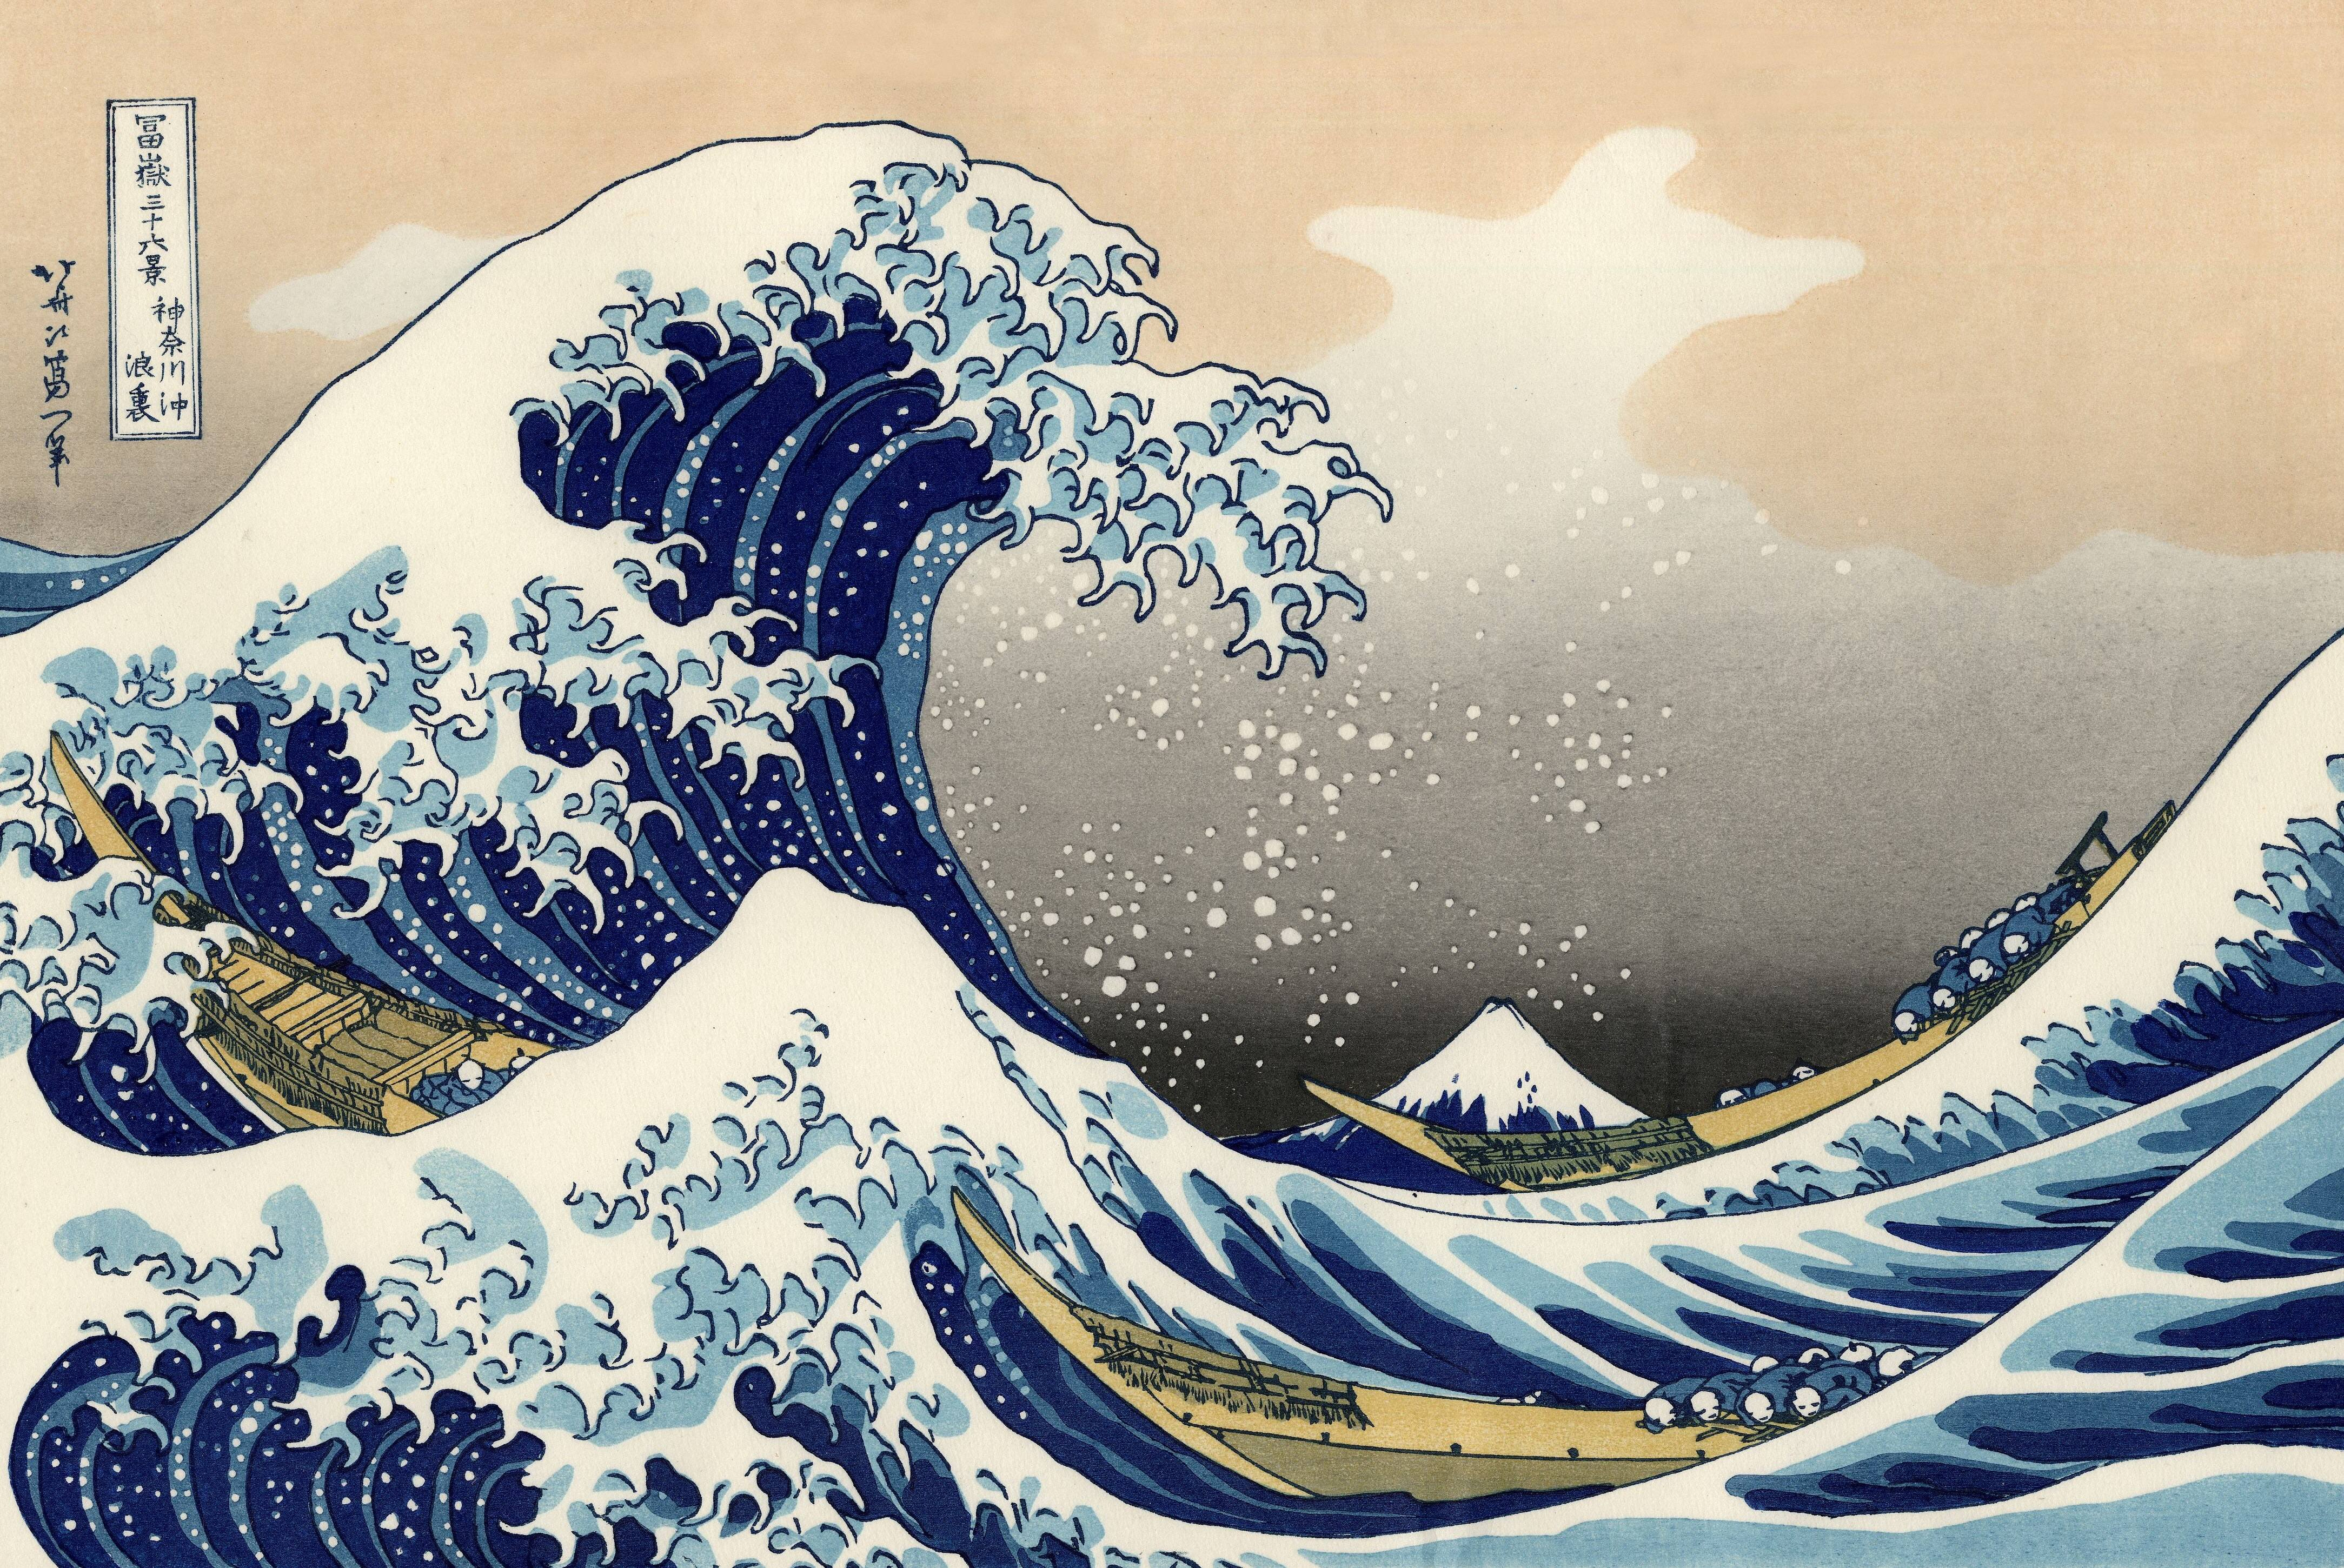
\includegraphics[width=\paperwidth, height=\paperwidth,keepaspectratio]{figures/background.png}}}

\begin{document}

	\maketitle
	\flushbottom
	\newpage
	\pagestyle{fancynotes}
	\part{引言}
    我从2019年9月就开始写这份笔记了,但写到今天也只有寥寥数页。原本的笔记也有这样一个引言部分,主要讲述了我整个大学四年的艰难历程,但现在看来,那些文字只不过是自己感动自己罢了\footnote{我仍然保留了那些文字,放在我的博客中:\href{https://shunzdai.now.sh/2020/06/04/My-Life-In-College/}{\textit{我的大学}}。}。现在,我重写了这份引言,用尽量简短的语言来阐述这份笔记做了些什么工作。
	
    这份笔记受微分几何的影响颇深,微分几何也是我大学四年以来尤其喜爱的数学领域。相比于线性代数,微分几何为代数问题赋予了几何的看法;相比于微积分(当然,我指的是高等数学中的微积分,而不是数学分析中的微积分),微分几何更注重“基本结构”,它没有繁多的运算技巧,不必将问题拘谨在冗长的计算中。事实上,理论物理与微分几何的关系可以说是“殊途同归”,它们都用到了公理化(或者说是“第一性原理”)的方法。在研究这种问题时,我们总可以从几条基本公理(或基本假设)出发,逐步推理出宏伟的结构。
    
    在繁琐冗长的计算训练中,我们逐步忘却了那些基本结构的作用。当然,这些论断不意味着我们在学习理论物理时不需要任何实际计算、应用,只是说,我们在学习理论物理时更应该将注意力放在基本结构上,而简单的计算能够加深理解,这就已经足够了,我们不必将精力放在如同上述第一个问题的复杂计算上。

    这份笔记中,我们将通篇使用Einstein求和约定,即相同的一对上下指标表示求和。我们将始终保持上下指标的差异,这种差异原则上与度量张量升降指标无关,而是一种源自事物本身的“对偶”属性。

    希望诸位能喜欢上本教程。
    
    $\quad$

    $\quad$

    \rightline{代顺治}
    \rightline{2020年10月31日,于深圳}
    
		\newpage
	\part{微分几何}\label{Part:Differential_Geometry}
	\begin{margintable}\vspace{1.4in}%\footnotesize
		\begin{tabularx}{\marginparwidth}{|X}
			Section~\ref{sec:Coordinates}. 局部坐标系\\
			%Section~\ref{sec:LieAlgebra}. 联络与曲率\\
			%Section~\ref{sec:Manifold}. 流形\\
		\end{tabularx}
	\end{margintable}
	内地的物理学工作者喜好在网络社区上整理自己的笔记.这些笔记虽然名义上被称作“笔记”,但实质上都只是抄书罢了.笔者不喜好抄书,也不喜好做笔记,但对于本章节的内容,笔者仍将大量参考Chern的讲义\upcite{bib:Chern01},并斗胆将这本书的所述内容改写成通俗的、适于家用的语言.当然,这样做会损失一些数学上的严谨,但笔者认为这无伤大雅.
	
	\section{坐标系}\label{sec:Coordinates}
	我们首先回顾一下线性空间的公理化定义.
		\begin{definition}
			域$F$上的线性空间$V$是这样一个集合,对任意$\alpha,\beta,\gamma\in V$;$a,b\in F$有
			\begin{enumerate}
				矢量加法映射$V\times V\rightarrow V$:
				\item (交换律)$\alpha+\beta=\beta+\alpha$;
				\item (结合律)$(\alpha+\beta)+\gamma=\alpha+(\beta+\gamma)$;
				\item (零元)存在唯一的$0\in V$,使得$0+\alpha=\alpha$;
				\item (逆元)对任意$\alpha\in V$,存在唯一的$\beta\in V$,使得$\alpha+\beta=0$.
					
				矢量数乘映射$F\times V\rightarrow V$:
				\item (酉性)对$1\in F$,有$1\alpha=\alpha$;
				\item (结合律)$a(b\alpha)=(ab)\alpha$;
				\item (分配律1)$(a+b)\alpha=a\alpha+b\alpha$;
				\item (分配律2)$a(\alpha+\beta)=a\alpha+a\beta$.
			\end{enumerate}
		\end{definition}
	在第一次学习这个定义的时候,你可能会问:“这有什么意义?交换律,结合律,分配律,这些东西不是小学就学了么?”这就是公理化的奇妙之处.我们总是能从这样通俗易懂的基础逻辑出发,演绎出宏伟的结构.数学是这样,后面我们会看到理论物理(而不是材料物理)也是这样.
			
	一个最平凡的例子就是$n$维Euclidean空间$\mathbb{R}^n$.我们将$\mathbb{R}^n$中的元素称为\textbf{点},记为一个有序数组$(x^1,\cdots,x^n)$,或简记为$(x^\mu),\mu=1,\cdots,n$,其中$x^\mu$是$n$个称为\textbf{坐标}的实参数.容易证明$\mathbb{R}^n$是一个实数域$\mathbb{R}$上的线性空间.
			
	事实上我们还可以引入不同的参数来表示空间中的同一点.例如,我们找来一组带撇的参数$x'^\mu$,然后将原来的$(x^1,\cdots,x^n)$转换为$(x'^1,\cdots,x'^n)$,这个过程称为\textbf{坐标变换},我们可以用一个映射$\varphi$表示之\footnote{通常会对这一映射加上某些光滑、可逆的限制.}:
	\begin{equation}\label{eq:coordinate transformation}
		\varphi:\mathbb{R}^n\rightarrow \mathbb{R}^n,(x^1,\cdots,x^n)\mapsto (x'^1,\cdots,x'^n).
	\end{equation}
	我们注意到(\ref{eq:coordinate transformation})这个映射相当于“输入$(x^1,\cdots,x^n)$,得到$x'^1$;$\cdots$;输入$(x^1,\cdots,x^n)$,得到$x'^n$”,而这等价于$n$个$n$元函数:
	\begin{equation}
		\begin{split}
			\varphi^1&:\mathbb{R}^n\rightarrow \mathbb{R},(x^1,\cdots,x^n)\mapsto x'^1;\\
			&\cdots\\
			\varphi^n&:\mathbb{R}^n\rightarrow \mathbb{R},(x^1,\cdots,x^n)\mapsto x'^n.
		\end{split}
	\end{equation}
	这就是通常意义下的坐标变换函数组.
			
	我们说,每一组参数组$(x^\mu)$都对应了一种参数坐标系.假设某组参数确定了一个$\mathbb{R}^n$中的点,当我们固定$n-1$个参数$x^{\mu_1},\cdots,x^{\mu_{i-1}},x^{\mu_{i+1}},\cdots,x^{\mu_n}$,只让一个参数$x^i$变化时,这个点就走出了一条轨迹.我们将这条轨迹称为坐标$x^i$的\textbf{坐标线}.对于$\mathbb{R}^3$,我们可以将坐标系画下来.
	\subsection{直角坐标系}
		\begin{marginfigure}
			\centering
			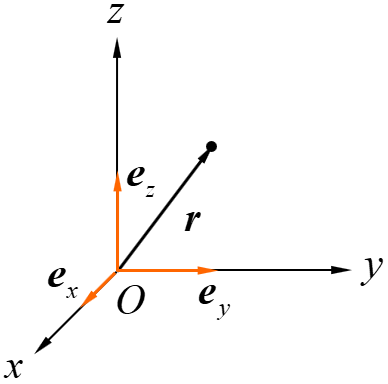
\includegraphics[width=1\textwidth]{figures/rectangular_coordinates.png}
			\caption{直角坐标系}\label{fig:rectangular_coordinates}
		\end{marginfigure}
	最典型的例子就是正交直角坐标系,或者说是Cartesian坐标系,如图\ref{fig:rectangular_coordinates}所示.在这种坐标系中,坐标线是直线,且彼此正交.通常,我们用$(x,y,z)$来表述直角坐标系中的点.
	\subsection{柱坐标系}
		\begin{marginfigure}
			\centering
			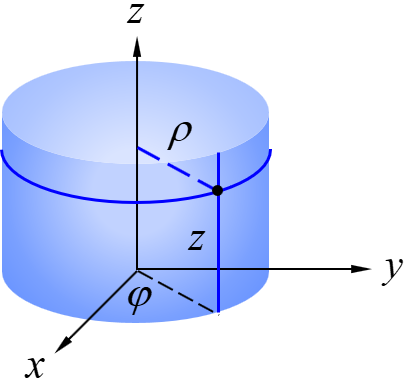
\includegraphics[width=1\textwidth]{figures/cylindrical_coordinates.png}
			\caption{柱坐标系}\label{fig:cylindrical_coordinates}
		\end{marginfigure}
		柱坐标系如图\ref{fig:cylindrical_coordinates}所示.通常,我们用$(r,\theta,z)$来表述柱坐标系中的点,其中线参数$r\in[0,+\infty)$,$z\in \mathbb{R}$,角参数$\theta\in[0,2\pi)$,这些参数构成的坐标线彼此正交.将一个由柱坐标参数描述的点变换到由直角坐标参数描述的点总是容易的,我们有它的坐标变换映射
		\begin{equation}\label{eq:rthetaz to xyz 1}
			(r,\theta,z)\mapsto(x,y,z),
		\end{equation}
		用坐标变换函数组表示就是
		\begin{equation}\label{eq:rthetaz to xyz 2}
			\begin{split}
				x(r,\theta,z)&=r\cos\theta;\\
				y(r,\theta,z)&=r\sin\theta;\\
				z(r,\theta,z)&=z.
			\end{split}
		\end{equation}
		我们注意到\ref{eq:rthetaz to xyz 2}是光滑的,这意味着它还是可逆的.于是我们可以得到\ref{eq:rthetaz to xyz 1}的逆映射
		\begin{equation}\label{eq:xyz to rthetaz 1}
			(x,y,z)\mapsto(r,\theta,z),
		\end{equation}
		用坐标变换函数组表示就是
		\begin{equation}\label{eq:xyz to rthetaz 2}
			\begin{split}
				r(x,y,z)&=\sqrt{x^2+y^2};\\
				\theta(x,y,z)&=\arccos\left(\frac{x}{\sqrt{x^2+y^2}}\right);\\
				z(x,y,z)&=z.
			\end{split}
		\end{equation}
			
	\subsection{球坐标系}
			
		\begin{marginfigure}
			\centering
			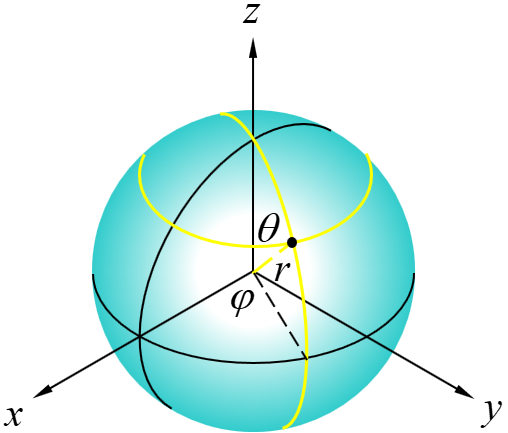
\includegraphics[width=1\textwidth]{figures/spherical_coordinates.png}
			\caption{球坐标系}\label{fig:spherical_coordinates}
		\end{marginfigure}
		球坐标系是除了直角坐标系以外最常用的坐标系,如图\ref{fig:spherical_coordinates}所示.我们用$(r,\theta,\varphi)$来描述球坐标系中的点,其中线参数$r\in[0,+\infty)$,角参数$\theta\in[0,\pi)$,$\varphi\in[0,2\pi)$,两个角参数通常隐含着系统的球对称性以及各向同性.与柱坐标系相同,球坐标系到直角坐标系也有坐标变换映射
		\begin{equation}\label{eq:rthetaphi to xyz 1}
			(r,\theta,\varphi)\mapsto(x,y,z),
		\end{equation}
		用坐标变换函数组表示就是
		\begin{equation}\label{eq:rthetaphi to xyz 2}
			\begin{split}
				x(r,\theta,\varphi)&=r\sin\theta \cos\varphi;\\
				y(r,\theta,\varphi)&=r\sin\theta \sin\varphi;\\
				z(r,\theta,\varphi)&=r\cos\theta.
			\end{split}
		\end{equation}
		同样的有直角坐标系到球坐标系的逆变换
		\begin{equation}\label{eq:xyz to rthetaphi 1}
			(r,\theta,\varphi)\mapsto(x,y,z),
		\end{equation}
		用坐标变换函数组表示就是
		\begin{equation}\label{eq:xyz to rthetaphi 2}
			\begin{split}
				r(x,y,z)&=\sqrt{x^2+y^2+z^2};\\
				\theta(x,y,z)&=\arccos\left(\frac{z}{\sqrt{x^2+y^2+z^2}}\right);\\
				\varphi(x,y,z)&=\arctan(\frac{y}{x}).
			\end{split}
		\end{equation}

		我还想再讲一讲超球坐标系,它是球坐标系进一步抽象的结果.$n$维的超球坐标系由$1$个线参数$x'^1\in[0,+\infty)$和$n-1$个角参数$x'^2,\cdots,x'^{n-2}\in[0,\pi)$,$x'^{n-1}\in[0,2\pi)$构成.超球坐标系到直角坐标系的坐标变换由如下映射给出
		\begin{equation}\label{eq:rthetaphi to xyz 3}
			\phi:R^n\rightarrow R^n;(x'^1,\cdots,x'^n)\mapsto(x^1,\cdots,x^n),
		\end{equation}
		用坐标变换函数组表示就是
		\begin{equation}\label{eq:rthetaphi to xyz 4}
			\begin{split}
				x^1(x'^1,\cdots,x'^n)&=x'^1\cos x'^2;\\
				x^2(x'^1,\cdots,x'^n)&=x'^1\sin x'^2\cos x'^3;\\
				x^3(x'^1,\cdots,x'^n)&=x'^1\sin x'^2\sin x'^3\cos x'^4;\\
				&\cdots\\
				x^{n-1}(x'^1,\cdots,x'^n)&=x'^1\sin x'^2\cdots \sin x'^{n-2}\cos x'^{n-1};\\
				x^{n}(x'^1,\cdots,x'^n)&=x'^1\sin x'^2\cdots \sin x'^{n-2}\sin x'^{n-1}.
			\end{split}
		\end{equation}
		如果我们令$n=3$,并进行参数变换$x^1=z$,$x^2=x$,$x^3=y$,以及$x'^1=r$,$x'^2=\theta$,$x'^3=\varphi$,则(\ref{eq:rthetaphi to xyz 4})就回到了(\ref{eq:rthetaphi to xyz 2})的情况.

		我们这就论述了三种常见的坐标系.这些坐标系都有一个特点,即坐标线相互垂直.通常我们也将这样的坐标系称为正交曲线坐标系.当然,还有其他的正交曲线坐标系,例如圆环坐标系、椭球坐标系,等等,我们不再一一列举.但你可能会问:“有没有坐标线相互不正交的曲线坐标系?”那么我的回答是:“当然有.”实际上,坐标线相互不正交的坐标系才是一般情况.为了描述一般情况下的坐标系,我们将坐标变换函数组统一的记成$x^\mu(x'^\nu)$的形式,其中$\mu$指标表示“取坐标变换函数组中的第$\mu$个函数$x^\mu$”,$\nu$指标表示“取定函数$x^\mu$后,取函数的第$\nu$个参数”.这样的表述方法称为\textbf{抽象指标}记号,抽象指标在取定数值后成为\textbf{具体指标}.后面我们会看到,这样的表述方法是非常方便的.
	%\section{由局部坐标系诱导的线性空间}
    欧式坐标诱导出两种特殊的线性空间,分别称为切空间和余切空间.我们可以定义线性空间与线性空间的“积”,从而构造出更大的线性空间,称为张量空间.另外,全反对称张量作为张量空间的特例具有特别的代数结构,称为外代数.本节将会一一讲述这些由欧式坐标诱导的线性空间.
    \subsection{切空间}
        \begin{definition}
            $\mathbb{R}^n$中的点$p$在坐标系$(x)$下的坐标为$(x^1,\cdots,x^n)$,则$(x^1,\cdots,x^n)$在$p$点诱导了一个线性空间$T_p\mathbb{R}^n$,$T_p\mathbb{R}^n$的元素即导数算符.
        \end{definition}
        我们将$T_p\mathbb{R}^n$称为切空间,$T_p\mathbb{R}^n$的元素称为切矢量.这个定义是说,任意一个切向量$X\in T_p\mathbb{R}^n$都能通过延坐标线的导数算符$\partial_\mu$在$p$点展开为
        \begin{equation}\label{eq:tangent 1}
            X=\left(X^\mu\frac{\partial}{\partial x^\mu}\right)\Bigg|_p,
        \end{equation}
        其中$x^\mu$表示切向量$X$在基底$\partial/\partial x^\mu$下的分量.我们也可以用矩阵显式写出(\ref{eq:tangent 1}),即
        \begin{equation}\label{eq:tangent 2}
            X=
            \begin{pmatrix}
                X^1&\cdots&X^n	
            \end{pmatrix}
            \begin{pmatrix}
                \frac{\partial}{\partial x^1}\\
                \vdots\\
                \frac{\partial}{\partial x^n}	
            \end{pmatrix}.
        \end{equation}
        在进行坐标变换时,切空间的基底像下面这样改变:
        \begin{equation}\label{eq:tangent 3}
            \frac{\partial}{\partial x^\mu}=\frac{\partial x'^\nu}{\partial x^\mu}\frac{\partial}{\partial x'^\nu},
        \end{equation}
        写成矩阵显式就是
        \begin{equation}\label{eq:tangent 4}
            \begin{pmatrix}
                \frac{\partial}{\partial x^1}\\
                \vdots\\
                \frac{\partial}{\partial x^n}	
            \end{pmatrix}
            =
            \begin{pmatrix}
                \frac{\partial x'^1}{\partial x^1}&\cdots&\frac{\partial x'^n}{\partial x^1}\\
                \vdots&\ddots&\vdots\\
                \frac{\partial x'^1}{\partial x^n}&\cdots&\frac{\partial x'^n}{\partial x^n}\\	
            \end{pmatrix}
            \begin{pmatrix}
                \frac{\partial}{\partial x'^1}\\
                \vdots\\
                \frac{\partial}{\partial x'^n}	
            \end{pmatrix}.
        \end{equation}
        我们将(\ref{eq:tangent 4})中产生的$n$阶方阵称为Jocobi矩阵,记为$J$.
        \begin{example}
            计算球坐标系下的切空间基底
            $\left(\frac{\partial}{\partial r}\ \frac{\partial}{\partial \theta}\ \frac{\partial}{\partial \varphi}\right)$
            转换到直角坐标系下的基底的变换关系.
            \begin{eqnarray*}
                \frac{\partial}{\partial r}&=&\frac{\partial x}{\partial r}\frac{\partial }{\partial x}+\frac{\partial y}{\partial r}\frac{\partial }{\partial y}+\frac{\partial z}{\partial r}\frac{\partial }{\partial z}=\sin\theta \cos\varphi\frac{\partial }{\partial x}+\sin\theta \sin\varphi\frac{\partial }{\partial y}+\cos\theta\frac{\partial }{\partial z};\\
                \frac{\partial}{\partial \theta}&=&\frac{\partial x}{\partial \theta}\frac{\partial }{\partial x}+\frac{\partial y}{\partial \theta}\frac{\partial }{\partial y}+\frac{\partial z}{\partial \theta}\frac{\partial }{\partial z}=r\cos\theta \cos\varphi\frac{\partial }{\partial x}+r\cos\theta \sin\varphi\frac{\partial }{\partial y}-r\sin\theta\frac{\partial }{\partial z};\\
                \frac{\partial}{\partial \varphi}&=&\frac{\partial x}{\partial \varphi}\frac{\partial }{\partial x}+\frac{\partial y}{\partial \varphi}\frac{\partial }{\partial y}+\frac{\partial z}{\partial \varphi}\frac{\partial }{\partial z}=-r\sin\theta \sin\varphi\frac{\partial }{\partial x}+r\sin\theta \cos\varphi\frac{\partial }{\partial y}.
            \end{eqnarray*}
            写成矩阵形式就是
            \begin{equation}
                \begin{pmatrix}
                    \frac{\partial}{\partial r}\\
                    \frac{\partial}{\partial \theta}\\
                    \frac{\partial}{\partial \varphi}	
                \end{pmatrix}
                =
                \begin{pmatrix}
                    \sin\theta \cos\varphi&\sin\theta \sin\varphi&\cos\theta\\
                    r\cos\theta \cos\varphi&r\cos\theta \sin\varphi&-r\sin\theta\\
                    -r\sin\theta \sin\varphi&r\sin\theta \cos\varphi&0\\	
                \end{pmatrix}
                \begin{pmatrix}
                    \frac{\partial}{\partial x}\\
                    \frac{\partial}{\partial y}\\
                    \frac{\partial}{\partial z}	
                \end{pmatrix}.
            \end{equation}
        \end{example}
        \begin{exercise}
            计算柱坐标系下的切空间基底
            $\left(\frac{\partial}{\partial r}\ \frac{\partial}{\partial \theta}\ \frac{\partial}{\partial z}\right)$
            转换到直角坐标系下的基底的变换关系.
        \end{exercise}
    \subsection{余切空间}
        \begin{definition}
            $\mathbb{R}^n$中的点$p$在坐标系$(x)$下的坐标为$(x^1,\cdots,x^n)$,则$(x^1,\cdots,x^n)$在$p$点诱导了一个线性空间$T_p^*\mathbb{R}^n$,$T_p^*\mathbb{R}^n$的元素即1微分形式.
        \end{definition}
        我们将$T_p^*\mathbb{R}^n$称为余切空间,$T_p^*\mathbb{R}^n$的元素称为余切矢量.这个定义是说,任意一个余切矢量$\omega\in T_p^*\mathbb{R}^n$都能通过延坐标线的微元$dx^\mu$在$p$点展开为
	%\section{什么是场}
	%\section{流形}\label{sec:Manifold}
	一个流形指的是这样一个结构,其在局部上是平直的,但整体不必是平直的.
	\subsection{Riemannian流形}
	%\section{联络}
	\subsection{仿射联络}
		对于任意标量场$\phi\in \varGamma(T_{(0,0)}M)$,其外微分$d\phi$仍是是一个张量场
		\begin{equation}
				 d\phi=\frac{\partial\phi}{\partial x^\mu}dx^\mu=\frac{\partial\phi}{\partial {x}^\mu}\frac{\partial{x}^\mu}{\partial {x'}^\nu}d{x'}^\nu=\frac{\partial{\phi'}}{\partial {x'}^\nu}d{x'}^\nu\in \varGamma(T_{(0,1)}M),
		\end{equation}
		这意味着$d\phi$仍是张量丛截面的元素,用学物理家的话来说也就是$d\phi$仍然满足张量的变换规律.
		
		一个自然的问题是,对于切矢量场或余切矢量场,其外微分是否仍然是张量丛截面的元素?但问题就出在这,外微分算子是一个定义在外形式丛截面上的线性算子,切矢量场不是外形式丛截面中的元素,因此我们无法对一个切矢量场求外微分;余切矢量场作为1微分形式场,虽然它是外形式丛截面的元素,但它只是一种全反对称的张量场,我们无法对一个一般的非全反对称张量场求外微分.这些困难意味着我们需要推广外微分算子,寻找一个定义在一般张量丛截面$\varGamma(T_{(p,q)}M)$上的线性微分算子,让我们能对那些不在外形式丛截面中的张量场进行“微分”运算.这样构造的线性微分算子就是\textbf{仿射联络}.
		\begin{remark}
		余切矢量场$\omega\in \varGamma(T_{(0,1)}M)$在局部坐标系改变时满足
		\begin{equation}\label{eq:domega1}
				\omega=\omega_\mu dx^\mu=\omega_\mu\frac{\partial{x}^\mu}{\partial {x'}^\nu}d{x'}^\nu=\omega'_\nu d{x'}^\nu,
		\end{equation}
		我们对(\ref{eq:domega1})求全微分得到
		\begin{eqnarray}\label{eq:domega2}
			d\omega &=&d\omega'_\nu{\wedge}d{x'}^\nu\notag\\
			&=&d\left(\omega_\mu\frac{\partial{x}^\mu}{{\partial}{x'}^\nu}\right)\wedge d{x'}^\nu\notag\\
			&=&\frac{\partial{x}^\mu}{{\partial}{x'}^\nu}d\omega_\mu{\wedge}d{x'}^\nu+\omega_{\mu}d\left(\frac{\partial{x}^\mu}{\partial {x'}^\nu}\right){\wedge}d{x'}^\nu\notag\\
			&=&\left(\frac{\partial{\omega}_\mu}{{\partial}{x}^\sigma}\frac{\partial{x}^\sigma}{\partial {x'}^\rho}\frac{\partial{x}^\mu}{{\partial}{x'}^\nu}+{\omega}_\mu\frac{\partial^2{x}^\mu}{\partial {x'}^\rho{\partial}{x'}^\nu}\right)d{x'}^\rho{\wedge}d{x'}^\nu\\
			&=&\frac{\partial\omega'_\nu}{{\partial}{x'}^\rho}d{x'}^\rho{\wedge}d{x'}^\nu\notag,
		\end{eqnarray}
		注意到\ref{eq:domega2}中产生了一个二阶偏微分项,与张量的变换规律对比可知,这一项破坏了张量的变换规律.但外微分形式场的全反对称特性可以消除掉这一项带来的影响,即
		\begin{eqnarray}
			\frac{\partial\omega'_\nu}{{\partial}{x'}^\rho}d{x'}^\rho{\wedge}d{x'}^\nu&=&2\partial'_{[\rho}\omega'_{\nu]}{dx'}^{\rho}\otimes{dx'}^\nu\notag\\
				&=&2\left(\partial_{[\sigma}\omega_{\mu]}\frac{\partial{x}^\sigma}{\partial {x'}^\rho}\frac{\partial{x}^\mu}{{\partial}{x'}^\nu}+{\omega}_\mu\frac{\partial^2{x}^\mu}{\partial {x'}^{[\rho}{\partial}{x'}^{\nu]}}\right){dx'}^{\rho}\otimes{dx'}^\nu\notag\\
			&=&2\partial_{[\sigma}\omega_{\mu]}\frac{\partial{x}^\sigma}{\partial {x'}^\rho}\frac{\partial{x}^\mu}{{\partial}{x'}^\nu}{dx'}^{\rho}\otimes{dx'}^\nu,
		\end{eqnarray}
		所以$d\omega$实际上仍是张量场.但微分形式场说到底只是一种特殊的全反对称张量场,对于一般的张量场,我们无法通过张量场自身的对称性消除上述二阶偏微分项.
		\end{remark}

		现代微分几何中的联络指的是一般矢量丛上的联络.这一节我们先讨论切丛$T_{(1,0)}(M)$上的联络(称为\textbf{仿射联络}),然后逐步构造出张量丛$T_{(p,q)}(M)$上的联络.下面,我们直接给出仿射联络的定义.
		\begin{definition}
			仿射联络是一个映射
			\begin{equation*}
				D:\varGamma(T_{(1,0)}M)\rightarrow \varGamma(T_{(1,1)}M),
			\end{equation*}
			它满足下列条件:
			\begin{enumerate}
				\item 对任意的$A,B\in \varGamma(T_{(1,0)}M)$有 D(A+B)=D(A)+D(B);						
				\item 对任意的$A\in \varGamma(T_{(1,0)}M),\alpha\in \varGamma(T_{(0,0)}M)$有$D(\alpha A)=d\alpha\otimes A+\alpha D(A)$.
			\end{enumerate}
		\end{definition}
		局部上,联络由一组1微分形式给出.我们先来看自然标架场$\{\partial_\mu\}$的联络,命
		\begin{equation}
		D(\partial_\mu)=\omega^\rho_\mu \otimes\partial_\rho={\varGamma^\rho}_{\mu\nu}dx^\nu\otimes \partial_\rho,
		\end{equation} 
		其中$\omega^\rho_\mu={\varGamma^\rho}_{\mu\nu}dx^\nu$,${\varGamma^\rho}_{\mu\nu}$称为\textbf{联络系数},它是局部坐标系中的光滑函数.将$\omega^\rho_\mu$作为矩阵$\omega$第$\rho$行第$\mu$列的元素,这样构造的矩阵$\omega$称为\textbf{联络方阵}.可见,任意两个联络间的差异完全体现在联络方阵上.现在,我们来看联络的变换规律.在标架变换下,由联络的定义立即得到
		\begin{eqnarray}
			D(\partial'_\nu)&=&D\left(\frac{\partial{x^\mu}}{\partial{x'}^\nu}{\partial}_\mu\right)\notag\\
			&=&d\left(\frac{\partial{x^\mu}}{\partial{x'}^\nu}\right)\otimes{\partial}_\mu+\frac{\partial{x^\mu}}{\partial{x'}^\nu}D\left({\partial}_\mu\right)\notag\\
			&=&\left[d\left(\frac{\partial{x^\rho}}{\partial{x'}^\nu}\right)+\frac{\partial{x^\mu}}{\partial{x'}^\nu}\omega^\rho_\mu\right]\otimes{\partial}_\rho\notag\\
			&=&\left[d\left(\frac{\partial{x^\rho}}{\partial{x'}^\nu}\right)\frac{\partial{{x'}^\sigma}}{\partial{x^\rho}}+\frac{\partial{x^\mu}}{\partial{x'}^\nu}\omega^\rho_\mu\frac{\partial{{x'}^\sigma}}{\partial{x^\rho}}\right]\otimes\partial'_\sigma\notag\\
			&=&{\omega'}^\sigma_\nu\otimes\partial'_\sigma,
		\end{eqnarray}
		其中
		\begin{equation}\label{eq:connection}
		{\omega'}^\sigma_\nu=d\left(\frac{\partial{x^\rho}}{\partial{x'}^\nu}\right)\frac{\partial{{x'}^\sigma}}{\partial{x^\rho}}+\frac{\partial{x^\mu}}{\partial{x'}^\nu}\omega^\rho_\mu\frac{\partial{{x'}^\sigma}}{\partial{x^\rho}},
		\end{equation}
		这就是联络方阵在局部标架场改变时的变换公式.我们还可以进一步展开(\ref{eq:connection}),得到
		\begin{equation}
		{{\varGamma'}^\sigma}_{\nu\lambda}=\frac{\partial^2{x^\rho}}{\partial{x'}^\lambda\partial{x'}^\nu}\frac{\partial{{x'}^\sigma}}{\partial{x^\rho}}+{\varGamma^\rho}_{\mu\alpha}\frac{\partial{x^\mu}}{\partial{x'}^\nu}\frac{\partial{x}^\alpha}{\partial{x'}^\lambda}\frac{\partial{{x'}^\sigma}}{\partial{x^\rho}},
		\end{equation}
		这正是通常意义下的联络变换公式.可见联络系数${\varGamma^\rho}_{\mu\nu}$并不是一个张量,但引入它能使$D(\partial_\mu)$遵循张量的变换规律.
		
		稍作思考可以发现,若使用全反对称化的技巧,我们也能利用联络系数构造出一个张量.我们将在稍后给出具体讨论.

		切丛截面的联络在余切丛截面上诱导出一个联络(仍记为$D$),易看出它是从$\varGamma(T_{(0,1)}M)$到\\$\varGamma(T_{(0,2)}M)$的映射.
		现在现在我们来考察$\{\partial_\mu\}$的对偶标架$\{dx^\mu\}$的联络.$D(dx^\mu)$由下式确定
		$$d\left(\partial_\mu,dx^\nu\right)=\left(D(\partial_\mu),dx^\nu\right)+\left(\partial_\mu,D(dx^\nu)\right),$$
		我们设
		$$D(dx^\nu)={\omega^*}^\nu_\rho\otimes{dx}^\rho,$$
		于是
		$$\left(\partial_\mu,D(dx^\nu)\right)=\left(\partial_\mu,{\omega^*}^\nu_\rho\otimes{dx}^\rho\right)={\omega^*}^\nu_\rho\delta^\rho_\mu={\omega^*}^\nu_\mu.$$
		考虑到对偶标架满足
		$$\left(\partial_\mu,dx^\nu\right)=\delta^\nu_\mu,$$ 
		于是得到
		\begin{eqnarray}
			{\omega^*}^\nu_\mu&=&\left(\partial_\mu,D(dx^\nu)\right)=-\left(D(\partial_\mu),dx^\nu\right)\\
				&=&-\left(\omega^\rho_\mu\otimes\partial_\rho,dx^\nu\right)=-{\omega}^\rho_\mu\delta^\nu_\rho=-{\omega}^\nu_\mu,
		\end{eqnarray}
		即
		$D(dx^\nu)=-{\omega}^\nu_\rho\otimes{dx}^\rho$.
		至此,我们就能计算任意$A\in T_{(1,0)}(M)$与$B\in T_{(0,1)}(M)$的联络了.在局部坐标系下,我们有:			\begin{eqnarray}
			\begin{split}
				D(A)&=D(A^\mu\partial_\mu)\\
				&=dA^\mu\otimes\partial_\mu+A^{\mu}D(\partial_\mu)\\
				&=(\partial_{\rho}A^\mu+A^{\nu}{\varGamma^\mu}_{\nu\rho})dx^\rho{\otimes}\partial_\mu\\
				&=\nabla_{\rho}A^{\mu}dx^\rho{\otimes}\partial_\mu;
			\end{split}
		\end{eqnarray}
		\begin{eqnarray}
			\begin{split}
				D(B)&=D(B_{\mu}{dx}^\mu)\\
				&=dB_\mu\otimes{dx}^\mu+B_{\mu}D({dx}^\mu)\\
				&=(\partial_{\rho}B_\mu-B_\nu{\varGamma^\nu}_{\mu\rho})dx^\rho{\otimes}dx^\mu\\
				&=\nabla_{\rho}B_{\mu}dx^\rho{\otimes}dx^\mu,
			\end{split}
		\end{eqnarray}
		其中
		\begin{eqnarray}
			\nabla_{\rho}A^\mu&=&\partial_{\rho}A^\mu+A^{\nu}{\varGamma^\mu}_{\nu\rho};\\
				\nabla_{\rho}B_{\mu}&=&\partial_{\rho}B_\mu-B_\nu{\varGamma^\nu}_{\mu\rho}.
		\end{eqnarray}							
		这正是通常意义下的\textbf{协变导数}运算.由此可见,协变导数是一种依赖于局部坐标系的分量表述.用类似的方法,我们能得到$T_{(p,q)}(M)$上的诱导联络.
		\begin{definition}在一般张量丛$T_{(p,q)}M$上,由仿射联络诱导的联络是一个映射
			$$D:\varGamma(T_{(p,q)}M)\rightarrow\varGamma(T_{(p,q+1)}M),$$
			设任意$S\in \varGamma(T_{(p,q)}M)$,则$S$的联络在局部坐标系下满足
			\begin{equation}
				\begin{split}
					D(S)&=D({S^{\mu_1\dots\mu_p}}_{\nu_1\dots\nu_q}\partial_{\mu_1}\otimes\dots\otimes\partial_{\mu_p}\otimes{dx}^{\nu_1}\otimes\dots\otimes{dx}^{\nu_q})\\
				%&=d({S^{\mu_1\dots\mu_p}}_{\nu_1\dots\nu_q})\otimes\partial_{\mu_1}\otimes\dots\otimes\partial_{\mu_p}\otimes{dx}^{\nu_1}\otimes\dots\otimes{dx}^{\nu_q}\notag\\
				%&+{S^{\mu_1\dots\mu_p}}_{\nu_1\dots\nu_q}D(\partial_{\mu_1})\otimes\dots\otimes\partial_{\mu_p}\otimes{dx}^{\nu_1}\otimes\dots\otimes{dx}^{\nu_q}\notag\\
				%&+\dots+{S^{\mu_1\dots\mu_p}}_{\nu_1\dots\nu_q}\partial_{\mu_1}\otimes\dots\otimes D({\partial_{\mu_p}})\otimes{dx}^{\nu_1}\otimes\dots\otimes{dx}^{\nu_q}\notag\\
				%&+{S^{\mu_1\dots\mu_p}}_{\nu_1\dots\nu_q}\partial_{\mu_1}\otimes\dots\otimes{\partial_{\mu_p}}\otimes D({dx}^{\nu_1})\otimes\dots\otimes{dx}^{\nu_q}\notag\\
				%&+\dots+{S^{\mu_1\dots\mu_p}}_{\nu_1\dots\nu_q}\partial_{\mu_1}\otimes\dots\otimes{\partial_{\mu_p}}\otimes{dx}^{\nu_1}\otimes\dots\otimes D({dx}^{\nu_q})\notag\\
				%&=(\partial_\rho{S^{\mu_1\dots\mu_p}}_{\nu_1\dots\nu_q}+{S^{\sigma\dots\mu_p}}_{\nu_1\dots\nu_q}{\varGamma^{\mu_1}}_{\sigma\rho}\notag\\
				%&+\dots+{S^{\mu_1\dots\sigma}}_{\nu_1\dots\nu_q}{\varGamma^{\mu_p}}_{\sigma\rho}-{S^{\mu_1\dots\mu_p}}_{\sigma\dots\nu_q}{\varGamma^{\sigma}}_{\nu_1\rho}\notag\\
				%&-\dots-{S^{\mu_1\dots\mu_p}}_{\nu_1\dots\sigma}{\varGamma^{\sigma}}_{\nu_q\rho})dx^\rho\otimes\partial_{\mu_1}\otimes\dots\otimes\partial_{\mu_p}\otimes{dx}^{\nu_1}\otimes\dots\otimes{dx}^{\nu_q}\notag\\
				&=\nabla_{\rho}{S^{\mu_1\dots\mu_p}}_{\nu_1\dots\nu_q}dx^\rho\otimes\partial_{\mu_1}\otimes\dots\otimes\partial_{\mu_p}\otimes{dx}^{\nu_1}\otimes\dots\otimes{dx}^{\nu_q},
				\end{split}
			\end{equation}
			其中
			\begin{equation}
				\begin{split}
					\nabla_{\rho}{S^{\mu_1\dots\mu_p}}_{\nu_1\dots\nu_q}&=\partial_\rho{S^{\mu_1\dots\mu_p}}_{\nu_1\dots\nu_q}\\
					&+{S^{\sigma\dots\mu_p}}_{\nu_1\dots\nu_q}{\varGamma^{\mu_1}}_{\sigma\rho}+\dots+{S^{\mu_1\dots\sigma}}_{\nu_1\dots\nu_q}{\varGamma^{\mu_p}}_{\sigma\rho}\\
					&-{S^{\mu_1\dots\mu_p}}_{\sigma\dots\nu_q}{\varGamma^{\sigma}}_{\nu_1\rho}-\dots-{S^{\mu_1\dots\mu_p}}_{\nu_1\dots\sigma}{\varGamma^{\sigma}}_{\nu_q\rho}.
				\end{split}		
			\end{equation}
		\end{definition}
    \subsection{Riemannian流形上的容许联络}
	\begin{thebibliography}{9}%宽度9
	\bibitem{bib:Chern01}陈省身,陈维桓.微分几何讲义[M].第二版.北京:北京大学出版社,2001
	\bibitem{bib:Chern02}陈维桓.微分流形初步[M].第二版.北京:高等教育出版社,2002
	\end{thebibliography}
		\section{坐标系}\label{sec:Coordinates}
	我们首先回顾一下线性空间的公理化定义.
		\begin{definition}
			域$F$上的线性空间$V$是这样一个集合,对任意$\alpha,\beta,\gamma\in V$;$a,b\in F$有
			\begin{enumerate}
				矢量加法映射$V\times V\rightarrow V$:
				\item (交换律)$\alpha+\beta=\beta+\alpha$;
				\item (结合律)$(\alpha+\beta)+\gamma=\alpha+(\beta+\gamma)$;
				\item (零元)存在唯一的$0\in V$,使得$0+\alpha=\alpha$;
				\item (逆元)对任意$\alpha\in V$,存在唯一的$\beta\in V$,使得$\alpha+\beta=0$.
					
				矢量数乘映射$F\times V\rightarrow V$:
				\item (酉性)对$1\in F$,有$1\alpha=\alpha$;
				\item (结合律)$a(b\alpha)=(ab)\alpha$;
				\item (分配律1)$(a+b)\alpha=a\alpha+b\alpha$;
				\item (分配律2)$a(\alpha+\beta)=a\alpha+a\beta$.
			\end{enumerate}
		\end{definition}
	在第一次学习这个定义的时候,你可能会问:“这有什么意义?交换律,结合律,分配律,这些东西不是小学就学了么?”这就是公理化的奇妙之处.我们总是能从这样通俗易懂的基础逻辑出发,演绎出宏伟的结构.数学是这样,后面我们会看到理论物理(而不是材料物理)也是这样.
			
	一个最平凡的例子就是$n$维Euclidean空间$\mathbb{R}^n$.我们将$\mathbb{R}^n$中的元素称为\textbf{点},记为一个有序数组$(x^1,\cdots,x^n)$,或简记为$(x^\mu),\mu=1,\cdots,n$,其中$x^\mu$是$n$个称为\textbf{坐标}的实参数.容易证明$\mathbb{R}^n$是一个实数域$\mathbb{R}$上的线性空间.
			
	事实上我们还可以引入不同的参数来表示空间中的同一点.例如,我们找来一组带撇的参数$x'^\mu$,然后将原来的$(x^1,\cdots,x^n)$转换为$(x'^1,\cdots,x'^n)$,这个过程称为\textbf{坐标变换},我们可以用一个映射$\varphi$表示之\footnote{通常会对这一映射加上某些光滑、可逆的限制.}:
	\begin{equation}\label{eq:coordinate transformation}
		\varphi:\mathbb{R}^n\rightarrow \mathbb{R}^n,(x^1,\cdots,x^n)\mapsto (x'^1,\cdots,x'^n).
	\end{equation}
	我们注意到(\ref{eq:coordinate transformation})这个映射相当于“输入$(x^1,\cdots,x^n)$,得到$x'^1$;$\cdots$;输入$(x^1,\cdots,x^n)$,得到$x'^n$”,而这等价于$n$个$n$元函数:
	\begin{equation}
		\begin{split}
			\varphi^1&:\mathbb{R}^n\rightarrow \mathbb{R},(x^1,\cdots,x^n)\mapsto x'^1;\\
			&\cdots\\
			\varphi^n&:\mathbb{R}^n\rightarrow \mathbb{R},(x^1,\cdots,x^n)\mapsto x'^n.
		\end{split}
	\end{equation}
	这就是通常意义下的坐标变换函数组.
			
	我们说,每一组参数组$(x^\mu)$都对应了一种参数坐标系.假设某组参数确定了一个$\mathbb{R}^n$中的点,当我们固定$n-1$个参数$x^{\mu_1},\cdots,x^{\mu_{i-1}},x^{\mu_{i+1}},\cdots,x^{\mu_n}$,只让一个参数$x^i$变化时,这个点就走出了一条轨迹.我们将这条轨迹称为坐标$x^i$的\textbf{坐标线}.对于$\mathbb{R}^3$,我们可以将坐标系画下来.
	\subsection{直角坐标系}
		\begin{marginfigure}
			\centering
			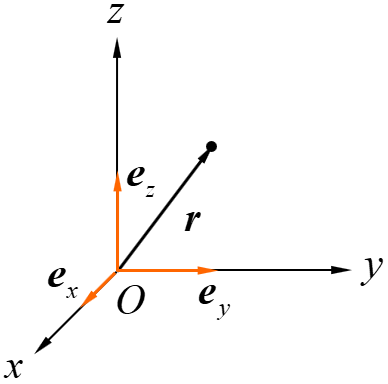
\includegraphics[width=1\textwidth]{figures/rectangular_coordinates.png}
			\caption{直角坐标系}\label{fig:rectangular_coordinates}
		\end{marginfigure}
	最典型的例子就是正交直角坐标系,或者说是Cartesian坐标系,如图\ref{fig:rectangular_coordinates}所示.在这种坐标系中,坐标线是直线,且彼此正交.通常,我们用$(x,y,z)$来表述直角坐标系中的点.
	\subsection{柱坐标系}
		\begin{marginfigure}
			\centering
			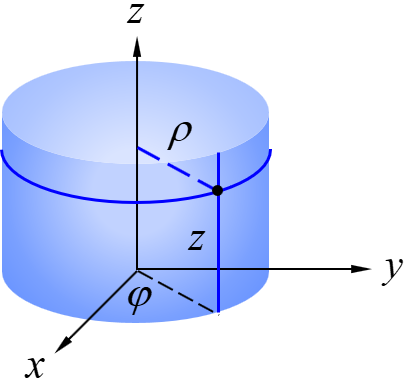
\includegraphics[width=1\textwidth]{figures/cylindrical_coordinates.png}
			\caption{柱坐标系}\label{fig:cylindrical_coordinates}
		\end{marginfigure}
		柱坐标系如图\ref{fig:cylindrical_coordinates}所示.通常,我们用$(r,\theta,z)$来表述柱坐标系中的点,其中线参数$r\in[0,+\infty)$,$z\in \mathbb{R}$,角参数$\theta\in[0,2\pi)$,这些参数构成的坐标线彼此正交.将一个由柱坐标参数描述的点变换到由直角坐标参数描述的点总是容易的,我们有它的坐标变换映射
		\begin{equation}\label{eq:rthetaz to xyz 1}
			(r,\theta,z)\mapsto(x,y,z),
		\end{equation}
		用坐标变换函数组表示就是
		\begin{equation}\label{eq:rthetaz to xyz 2}
			\begin{split}
				x(r,\theta,z)&=r\cos\theta;\\
				y(r,\theta,z)&=r\sin\theta;\\
				z(r,\theta,z)&=z.
			\end{split}
		\end{equation}
		我们注意到\ref{eq:rthetaz to xyz 2}是光滑的,这意味着它还是可逆的.于是我们可以得到\ref{eq:rthetaz to xyz 1}的逆映射
		\begin{equation}\label{eq:xyz to rthetaz 1}
			(x,y,z)\mapsto(r,\theta,z),
		\end{equation}
		用坐标变换函数组表示就是
		\begin{equation}\label{eq:xyz to rthetaz 2}
			\begin{split}
				r(x,y,z)&=\sqrt{x^2+y^2};\\
				\theta(x,y,z)&=\arccos\left(\frac{x}{\sqrt{x^2+y^2}}\right);\\
				z(x,y,z)&=z.
			\end{split}
		\end{equation}
			
	\subsection{球坐标系}
			
		\begin{marginfigure}
			\centering
			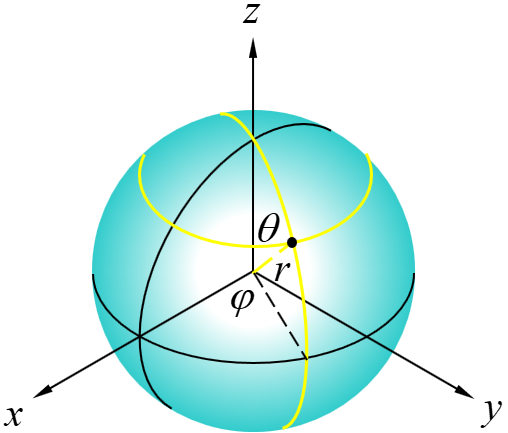
\includegraphics[width=1\textwidth]{figures/spherical_coordinates.png}
			\caption{球坐标系}\label{fig:spherical_coordinates}
		\end{marginfigure}
		球坐标系是除了直角坐标系以外最常用的坐标系,如图\ref{fig:spherical_coordinates}所示.我们用$(r,\theta,\varphi)$来描述球坐标系中的点,其中线参数$r\in[0,+\infty)$,角参数$\theta\in[0,\pi)$,$\varphi\in[0,2\pi)$,两个角参数通常隐含着系统的球对称性以及各向同性.与柱坐标系相同,球坐标系到直角坐标系也有坐标变换映射
		\begin{equation}\label{eq:rthetaphi to xyz 1}
			(r,\theta,\varphi)\mapsto(x,y,z),
		\end{equation}
		用坐标变换函数组表示就是
		\begin{equation}\label{eq:rthetaphi to xyz 2}
			\begin{split}
				x(r,\theta,\varphi)&=r\sin\theta \cos\varphi;\\
				y(r,\theta,\varphi)&=r\sin\theta \sin\varphi;\\
				z(r,\theta,\varphi)&=r\cos\theta.
			\end{split}
		\end{equation}
		同样的有直角坐标系到球坐标系的逆变换
		\begin{equation}\label{eq:xyz to rthetaphi 1}
			(r,\theta,\varphi)\mapsto(x,y,z),
		\end{equation}
		用坐标变换函数组表示就是
		\begin{equation}\label{eq:xyz to rthetaphi 2}
			\begin{split}
				r(x,y,z)&=\sqrt{x^2+y^2+z^2};\\
				\theta(x,y,z)&=\arccos\left(\frac{z}{\sqrt{x^2+y^2+z^2}}\right);\\
				\varphi(x,y,z)&=\arctan(\frac{y}{x}).
			\end{split}
		\end{equation}

		我还想再讲一讲超球坐标系,它是球坐标系进一步抽象的结果.$n$维的超球坐标系由$1$个线参数$x'^1\in[0,+\infty)$和$n-1$个角参数$x'^2,\cdots,x'^{n-2}\in[0,\pi)$,$x'^{n-1}\in[0,2\pi)$构成.超球坐标系到直角坐标系的坐标变换由如下映射给出
		\begin{equation}\label{eq:rthetaphi to xyz 3}
			\phi:R^n\rightarrow R^n;(x'^1,\cdots,x'^n)\mapsto(x^1,\cdots,x^n),
		\end{equation}
		用坐标变换函数组表示就是
		\begin{equation}\label{eq:rthetaphi to xyz 4}
			\begin{split}
				x^1(x'^1,\cdots,x'^n)&=x'^1\cos x'^2;\\
				x^2(x'^1,\cdots,x'^n)&=x'^1\sin x'^2\cos x'^3;\\
				x^3(x'^1,\cdots,x'^n)&=x'^1\sin x'^2\sin x'^3\cos x'^4;\\
				&\cdots\\
				x^{n-1}(x'^1,\cdots,x'^n)&=x'^1\sin x'^2\cdots \sin x'^{n-2}\cos x'^{n-1};\\
				x^{n}(x'^1,\cdots,x'^n)&=x'^1\sin x'^2\cdots \sin x'^{n-2}\sin x'^{n-1}.
			\end{split}
		\end{equation}
		如果我们令$n=3$,并进行参数变换$x^1=z$,$x^2=x$,$x^3=y$,以及$x'^1=r$,$x'^2=\theta$,$x'^3=\varphi$,则(\ref{eq:rthetaphi to xyz 4})就回到了(\ref{eq:rthetaphi to xyz 2})的情况.

		我们这就论述了三种常见的坐标系.这些坐标系都有一个特点,即坐标线相互垂直.通常我们也将这样的坐标系称为正交曲线坐标系.当然,还有其他的正交曲线坐标系,例如圆环坐标系、椭球坐标系,等等,我们不再一一列举.但你可能会问:“有没有坐标线相互不正交的曲线坐标系?”那么我的回答是:“当然有.”实际上,坐标线相互不正交的坐标系才是一般情况.为了描述一般情况下的坐标系,我们将坐标变换函数组统一的记成$x^\mu(x'^\nu)$的形式,其中$\mu$指标表示“取坐标变换函数组中的第$\mu$个函数$x^\mu$”,$\nu$指标表示“取定函数$x^\mu$后,取函数的第$\nu$个参数”.这样的表述方法称为\textbf{抽象指标}记号,抽象指标在取定数值后成为\textbf{具体指标}.后面我们会看到,这样的表述方法是非常方便的.
		\section{由局部坐标系诱导的线性空间}
    欧式坐标诱导出两种特殊的线性空间,分别称为切空间和余切空间.我们可以定义线性空间与线性空间的“积”,从而构造出更大的线性空间,称为张量空间.另外,全反对称张量作为张量空间的特例具有特别的代数结构,称为外代数.本节将会一一讲述这些由欧式坐标诱导的线性空间.
    \subsection{切空间}
        \begin{definition}
            $\mathbb{R}^n$中的点$p$在坐标系$(x)$下的坐标为$(x^1,\cdots,x^n)$,则$(x^1,\cdots,x^n)$在$p$点诱导了一个线性空间$T_p\mathbb{R}^n$,$T_p\mathbb{R}^n$的元素即导数算符.
        \end{definition}
        我们将$T_p\mathbb{R}^n$称为切空间,$T_p\mathbb{R}^n$的元素称为切矢量.这个定义是说,任意一个切向量$X\in T_p\mathbb{R}^n$都能通过延坐标线的导数算符$\partial_\mu$在$p$点展开为
        \begin{equation}\label{eq:tangent 1}
            X=\left(X^\mu\frac{\partial}{\partial x^\mu}\right)\Bigg|_p,
        \end{equation}
        其中$x^\mu$表示切向量$X$在基底$\partial/\partial x^\mu$下的分量.我们也可以用矩阵显式写出(\ref{eq:tangent 1}),即
        \begin{equation}\label{eq:tangent 2}
            X=
            \begin{pmatrix}
                X^1&\cdots&X^n	
            \end{pmatrix}
            \begin{pmatrix}
                \frac{\partial}{\partial x^1}\\
                \vdots\\
                \frac{\partial}{\partial x^n}	
            \end{pmatrix}.
        \end{equation}
        在进行坐标变换时,切空间的基底像下面这样改变:
        \begin{equation}\label{eq:tangent 3}
            \frac{\partial}{\partial x^\mu}=\frac{\partial x'^\nu}{\partial x^\mu}\frac{\partial}{\partial x'^\nu},
        \end{equation}
        写成矩阵显式就是
        \begin{equation}\label{eq:tangent 4}
            \begin{pmatrix}
                \frac{\partial}{\partial x^1}\\
                \vdots\\
                \frac{\partial}{\partial x^n}	
            \end{pmatrix}
            =
            \begin{pmatrix}
                \frac{\partial x'^1}{\partial x^1}&\cdots&\frac{\partial x'^n}{\partial x^1}\\
                \vdots&\ddots&\vdots\\
                \frac{\partial x'^1}{\partial x^n}&\cdots&\frac{\partial x'^n}{\partial x^n}\\	
            \end{pmatrix}
            \begin{pmatrix}
                \frac{\partial}{\partial x'^1}\\
                \vdots\\
                \frac{\partial}{\partial x'^n}	
            \end{pmatrix}.
        \end{equation}
        我们将(\ref{eq:tangent 4})中产生的$n$阶方阵称为Jocobi矩阵,记为$J$.
        \begin{example}
            计算球坐标系下的切空间基底
            $\left(\frac{\partial}{\partial r}\ \frac{\partial}{\partial \theta}\ \frac{\partial}{\partial \varphi}\right)$
            转换到直角坐标系下的基底的变换关系.
            \begin{eqnarray*}
                \frac{\partial}{\partial r}&=&\frac{\partial x}{\partial r}\frac{\partial }{\partial x}+\frac{\partial y}{\partial r}\frac{\partial }{\partial y}+\frac{\partial z}{\partial r}\frac{\partial }{\partial z}=\sin\theta \cos\varphi\frac{\partial }{\partial x}+\sin\theta \sin\varphi\frac{\partial }{\partial y}+\cos\theta\frac{\partial }{\partial z};\\
                \frac{\partial}{\partial \theta}&=&\frac{\partial x}{\partial \theta}\frac{\partial }{\partial x}+\frac{\partial y}{\partial \theta}\frac{\partial }{\partial y}+\frac{\partial z}{\partial \theta}\frac{\partial }{\partial z}=r\cos\theta \cos\varphi\frac{\partial }{\partial x}+r\cos\theta \sin\varphi\frac{\partial }{\partial y}-r\sin\theta\frac{\partial }{\partial z};\\
                \frac{\partial}{\partial \varphi}&=&\frac{\partial x}{\partial \varphi}\frac{\partial }{\partial x}+\frac{\partial y}{\partial \varphi}\frac{\partial }{\partial y}+\frac{\partial z}{\partial \varphi}\frac{\partial }{\partial z}=-r\sin\theta \sin\varphi\frac{\partial }{\partial x}+r\sin\theta \cos\varphi\frac{\partial }{\partial y}.
            \end{eqnarray*}
            写成矩阵形式就是
            \begin{equation}
                \begin{pmatrix}
                    \frac{\partial}{\partial r}\\
                    \frac{\partial}{\partial \theta}\\
                    \frac{\partial}{\partial \varphi}	
                \end{pmatrix}
                =
                \begin{pmatrix}
                    \sin\theta \cos\varphi&\sin\theta \sin\varphi&\cos\theta\\
                    r\cos\theta \cos\varphi&r\cos\theta \sin\varphi&-r\sin\theta\\
                    -r\sin\theta \sin\varphi&r\sin\theta \cos\varphi&0\\	
                \end{pmatrix}
                \begin{pmatrix}
                    \frac{\partial}{\partial x}\\
                    \frac{\partial}{\partial y}\\
                    \frac{\partial}{\partial z}	
                \end{pmatrix}.
            \end{equation}
        \end{example}
        \begin{exercise}
            计算柱坐标系下的切空间基底
            $\left(\frac{\partial}{\partial r}\ \frac{\partial}{\partial \theta}\ \frac{\partial}{\partial z}\right)$
            转换到直角坐标系下的基底的变换关系.
        \end{exercise}
    \subsection{余切空间}
        \begin{definition}
            $\mathbb{R}^n$中的点$p$在坐标系$(x)$下的坐标为$(x^1,\cdots,x^n)$,则$(x^1,\cdots,x^n)$在$p$点诱导了一个线性空间$T_p^*\mathbb{R}^n$,$T_p^*\mathbb{R}^n$的元素即1微分形式.
        \end{definition}
        我们将$T_p^*\mathbb{R}^n$称为余切空间,$T_p^*\mathbb{R}^n$的元素称为余切矢量.这个定义是说,任意一个余切矢量$\omega\in T_p^*\mathbb{R}^n$都能通过延坐标线的微元$dx^\mu$在$p$点展开为
		\section{什么是场}
		\section{流形}\label{sec:Manifold}
	一个流形指的是这样一个结构,其在局部上是平直的,但整体不必是平直的.
	\subsection{Riemannian流形}
		\section{联络}
	\subsection{仿射联络}
		对于任意标量场$\phi\in \varGamma(T_{(0,0)}M)$,其外微分$d\phi$仍是是一个张量场
		\begin{equation}
				 d\phi=\frac{\partial\phi}{\partial x^\mu}dx^\mu=\frac{\partial\phi}{\partial {x}^\mu}\frac{\partial{x}^\mu}{\partial {x'}^\nu}d{x'}^\nu=\frac{\partial{\phi'}}{\partial {x'}^\nu}d{x'}^\nu\in \varGamma(T_{(0,1)}M),
		\end{equation}
		这意味着$d\phi$仍是张量丛截面的元素,用学物理家的话来说也就是$d\phi$仍然满足张量的变换规律.
		
		一个自然的问题是,对于切矢量场或余切矢量场,其外微分是否仍然是张量丛截面的元素?但问题就出在这,外微分算子是一个定义在外形式丛截面上的线性算子,切矢量场不是外形式丛截面中的元素,因此我们无法对一个切矢量场求外微分;余切矢量场作为1微分形式场,虽然它是外形式丛截面的元素,但它只是一种全反对称的张量场,我们无法对一个一般的非全反对称张量场求外微分.这些困难意味着我们需要推广外微分算子,寻找一个定义在一般张量丛截面$\varGamma(T_{(p,q)}M)$上的线性微分算子,让我们能对那些不在外形式丛截面中的张量场进行“微分”运算.这样构造的线性微分算子就是\textbf{仿射联络}.
		\begin{remark}
		余切矢量场$\omega\in \varGamma(T_{(0,1)}M)$在局部坐标系改变时满足
		\begin{equation}\label{eq:domega1}
				\omega=\omega_\mu dx^\mu=\omega_\mu\frac{\partial{x}^\mu}{\partial {x'}^\nu}d{x'}^\nu=\omega'_\nu d{x'}^\nu,
		\end{equation}
		我们对(\ref{eq:domega1})求全微分得到
		\begin{eqnarray}\label{eq:domega2}
			d\omega &=&d\omega'_\nu{\wedge}d{x'}^\nu\notag\\
			&=&d\left(\omega_\mu\frac{\partial{x}^\mu}{{\partial}{x'}^\nu}\right)\wedge d{x'}^\nu\notag\\
			&=&\frac{\partial{x}^\mu}{{\partial}{x'}^\nu}d\omega_\mu{\wedge}d{x'}^\nu+\omega_{\mu}d\left(\frac{\partial{x}^\mu}{\partial {x'}^\nu}\right){\wedge}d{x'}^\nu\notag\\
			&=&\left(\frac{\partial{\omega}_\mu}{{\partial}{x}^\sigma}\frac{\partial{x}^\sigma}{\partial {x'}^\rho}\frac{\partial{x}^\mu}{{\partial}{x'}^\nu}+{\omega}_\mu\frac{\partial^2{x}^\mu}{\partial {x'}^\rho{\partial}{x'}^\nu}\right)d{x'}^\rho{\wedge}d{x'}^\nu\\
			&=&\frac{\partial\omega'_\nu}{{\partial}{x'}^\rho}d{x'}^\rho{\wedge}d{x'}^\nu\notag,
		\end{eqnarray}
		注意到\ref{eq:domega2}中产生了一个二阶偏微分项,与张量的变换规律对比可知,这一项破坏了张量的变换规律.但外微分形式场的全反对称特性可以消除掉这一项带来的影响,即
		\begin{eqnarray}
			\frac{\partial\omega'_\nu}{{\partial}{x'}^\rho}d{x'}^\rho{\wedge}d{x'}^\nu&=&2\partial'_{[\rho}\omega'_{\nu]}{dx'}^{\rho}\otimes{dx'}^\nu\notag\\
				&=&2\left(\partial_{[\sigma}\omega_{\mu]}\frac{\partial{x}^\sigma}{\partial {x'}^\rho}\frac{\partial{x}^\mu}{{\partial}{x'}^\nu}+{\omega}_\mu\frac{\partial^2{x}^\mu}{\partial {x'}^{[\rho}{\partial}{x'}^{\nu]}}\right){dx'}^{\rho}\otimes{dx'}^\nu\notag\\
			&=&2\partial_{[\sigma}\omega_{\mu]}\frac{\partial{x}^\sigma}{\partial {x'}^\rho}\frac{\partial{x}^\mu}{{\partial}{x'}^\nu}{dx'}^{\rho}\otimes{dx'}^\nu,
		\end{eqnarray}
		所以$d\omega$实际上仍是张量场.但微分形式场说到底只是一种特殊的全反对称张量场,对于一般的张量场,我们无法通过张量场自身的对称性消除上述二阶偏微分项.
		\end{remark}

		现代微分几何中的联络指的是一般矢量丛上的联络.这一节我们先讨论切丛$T_{(1,0)}(M)$上的联络(称为\textbf{仿射联络}),然后逐步构造出张量丛$T_{(p,q)}(M)$上的联络.下面,我们直接给出仿射联络的定义.
		\begin{definition}
			仿射联络是一个映射
			\begin{equation*}
				D:\varGamma(T_{(1,0)}M)\rightarrow \varGamma(T_{(1,1)}M),
			\end{equation*}
			它满足下列条件:
			\begin{enumerate}
				\item 对任意的$A,B\in \varGamma(T_{(1,0)}M)$有 D(A+B)=D(A)+D(B);						
				\item 对任意的$A\in \varGamma(T_{(1,0)}M),\alpha\in \varGamma(T_{(0,0)}M)$有$D(\alpha A)=d\alpha\otimes A+\alpha D(A)$.
			\end{enumerate}
		\end{definition}
		局部上,联络由一组1微分形式给出.我们先来看自然标架场$\{\partial_\mu\}$的联络,命
		\begin{equation}
		D(\partial_\mu)=\omega^\rho_\mu \otimes\partial_\rho={\varGamma^\rho}_{\mu\nu}dx^\nu\otimes \partial_\rho,
		\end{equation} 
		其中$\omega^\rho_\mu={\varGamma^\rho}_{\mu\nu}dx^\nu$,${\varGamma^\rho}_{\mu\nu}$称为\textbf{联络系数},它是局部坐标系中的光滑函数.将$\omega^\rho_\mu$作为矩阵$\omega$第$\rho$行第$\mu$列的元素,这样构造的矩阵$\omega$称为\textbf{联络方阵}.可见,任意两个联络间的差异完全体现在联络方阵上.现在,我们来看联络的变换规律.在标架变换下,由联络的定义立即得到
		\begin{eqnarray}
			D(\partial'_\nu)&=&D\left(\frac{\partial{x^\mu}}{\partial{x'}^\nu}{\partial}_\mu\right)\notag\\
			&=&d\left(\frac{\partial{x^\mu}}{\partial{x'}^\nu}\right)\otimes{\partial}_\mu+\frac{\partial{x^\mu}}{\partial{x'}^\nu}D\left({\partial}_\mu\right)\notag\\
			&=&\left[d\left(\frac{\partial{x^\rho}}{\partial{x'}^\nu}\right)+\frac{\partial{x^\mu}}{\partial{x'}^\nu}\omega^\rho_\mu\right]\otimes{\partial}_\rho\notag\\
			&=&\left[d\left(\frac{\partial{x^\rho}}{\partial{x'}^\nu}\right)\frac{\partial{{x'}^\sigma}}{\partial{x^\rho}}+\frac{\partial{x^\mu}}{\partial{x'}^\nu}\omega^\rho_\mu\frac{\partial{{x'}^\sigma}}{\partial{x^\rho}}\right]\otimes\partial'_\sigma\notag\\
			&=&{\omega'}^\sigma_\nu\otimes\partial'_\sigma,
		\end{eqnarray}
		其中
		\begin{equation}\label{eq:connection}
		{\omega'}^\sigma_\nu=d\left(\frac{\partial{x^\rho}}{\partial{x'}^\nu}\right)\frac{\partial{{x'}^\sigma}}{\partial{x^\rho}}+\frac{\partial{x^\mu}}{\partial{x'}^\nu}\omega^\rho_\mu\frac{\partial{{x'}^\sigma}}{\partial{x^\rho}},
		\end{equation}
		这就是联络方阵在局部标架场改变时的变换公式.我们还可以进一步展开(\ref{eq:connection}),得到
		\begin{equation}
		{{\varGamma'}^\sigma}_{\nu\lambda}=\frac{\partial^2{x^\rho}}{\partial{x'}^\lambda\partial{x'}^\nu}\frac{\partial{{x'}^\sigma}}{\partial{x^\rho}}+{\varGamma^\rho}_{\mu\alpha}\frac{\partial{x^\mu}}{\partial{x'}^\nu}\frac{\partial{x}^\alpha}{\partial{x'}^\lambda}\frac{\partial{{x'}^\sigma}}{\partial{x^\rho}},
		\end{equation}
		这正是通常意义下的联络变换公式.可见联络系数${\varGamma^\rho}_{\mu\nu}$并不是一个张量,但引入它能使$D(\partial_\mu)$遵循张量的变换规律.
		
		稍作思考可以发现,若使用全反对称化的技巧,我们也能利用联络系数构造出一个张量.我们将在稍后给出具体讨论.

		切丛截面的联络在余切丛截面上诱导出一个联络(仍记为$D$),易看出它是从$\varGamma(T_{(0,1)}M)$到\\$\varGamma(T_{(0,2)}M)$的映射.
		现在现在我们来考察$\{\partial_\mu\}$的对偶标架$\{dx^\mu\}$的联络.$D(dx^\mu)$由下式确定
		$$d\left(\partial_\mu,dx^\nu\right)=\left(D(\partial_\mu),dx^\nu\right)+\left(\partial_\mu,D(dx^\nu)\right),$$
		我们设
		$$D(dx^\nu)={\omega^*}^\nu_\rho\otimes{dx}^\rho,$$
		于是
		$$\left(\partial_\mu,D(dx^\nu)\right)=\left(\partial_\mu,{\omega^*}^\nu_\rho\otimes{dx}^\rho\right)={\omega^*}^\nu_\rho\delta^\rho_\mu={\omega^*}^\nu_\mu.$$
		考虑到对偶标架满足
		$$\left(\partial_\mu,dx^\nu\right)=\delta^\nu_\mu,$$ 
		于是得到
		\begin{eqnarray}
			{\omega^*}^\nu_\mu&=&\left(\partial_\mu,D(dx^\nu)\right)=-\left(D(\partial_\mu),dx^\nu\right)\\
				&=&-\left(\omega^\rho_\mu\otimes\partial_\rho,dx^\nu\right)=-{\omega}^\rho_\mu\delta^\nu_\rho=-{\omega}^\nu_\mu,
		\end{eqnarray}
		即
		$D(dx^\nu)=-{\omega}^\nu_\rho\otimes{dx}^\rho$.
		至此,我们就能计算任意$A\in T_{(1,0)}(M)$与$B\in T_{(0,1)}(M)$的联络了.在局部坐标系下,我们有:			\begin{eqnarray}
			\begin{split}
				D(A)&=D(A^\mu\partial_\mu)\\
				&=dA^\mu\otimes\partial_\mu+A^{\mu}D(\partial_\mu)\\
				&=(\partial_{\rho}A^\mu+A^{\nu}{\varGamma^\mu}_{\nu\rho})dx^\rho{\otimes}\partial_\mu\\
				&=\nabla_{\rho}A^{\mu}dx^\rho{\otimes}\partial_\mu;
			\end{split}
		\end{eqnarray}
		\begin{eqnarray}
			\begin{split}
				D(B)&=D(B_{\mu}{dx}^\mu)\\
				&=dB_\mu\otimes{dx}^\mu+B_{\mu}D({dx}^\mu)\\
				&=(\partial_{\rho}B_\mu-B_\nu{\varGamma^\nu}_{\mu\rho})dx^\rho{\otimes}dx^\mu\\
				&=\nabla_{\rho}B_{\mu}dx^\rho{\otimes}dx^\mu,
			\end{split}
		\end{eqnarray}
		其中
		\begin{eqnarray}
			\nabla_{\rho}A^\mu&=&\partial_{\rho}A^\mu+A^{\nu}{\varGamma^\mu}_{\nu\rho};\\
				\nabla_{\rho}B_{\mu}&=&\partial_{\rho}B_\mu-B_\nu{\varGamma^\nu}_{\mu\rho}.
		\end{eqnarray}							
		这正是通常意义下的\textbf{协变导数}运算.由此可见,协变导数是一种依赖于局部坐标系的分量表述.用类似的方法,我们能得到$T_{(p,q)}(M)$上的诱导联络.
		\begin{definition}在一般张量丛$T_{(p,q)}M$上,由仿射联络诱导的联络是一个映射
			$$D:\varGamma(T_{(p,q)}M)\rightarrow\varGamma(T_{(p,q+1)}M),$$
			设任意$S\in \varGamma(T_{(p,q)}M)$,则$S$的联络在局部坐标系下满足
			\begin{equation}
				\begin{split}
					D(S)&=D({S^{\mu_1\dots\mu_p}}_{\nu_1\dots\nu_q}\partial_{\mu_1}\otimes\dots\otimes\partial_{\mu_p}\otimes{dx}^{\nu_1}\otimes\dots\otimes{dx}^{\nu_q})\\
				%&=d({S^{\mu_1\dots\mu_p}}_{\nu_1\dots\nu_q})\otimes\partial_{\mu_1}\otimes\dots\otimes\partial_{\mu_p}\otimes{dx}^{\nu_1}\otimes\dots\otimes{dx}^{\nu_q}\notag\\
				%&+{S^{\mu_1\dots\mu_p}}_{\nu_1\dots\nu_q}D(\partial_{\mu_1})\otimes\dots\otimes\partial_{\mu_p}\otimes{dx}^{\nu_1}\otimes\dots\otimes{dx}^{\nu_q}\notag\\
				%&+\dots+{S^{\mu_1\dots\mu_p}}_{\nu_1\dots\nu_q}\partial_{\mu_1}\otimes\dots\otimes D({\partial_{\mu_p}})\otimes{dx}^{\nu_1}\otimes\dots\otimes{dx}^{\nu_q}\notag\\
				%&+{S^{\mu_1\dots\mu_p}}_{\nu_1\dots\nu_q}\partial_{\mu_1}\otimes\dots\otimes{\partial_{\mu_p}}\otimes D({dx}^{\nu_1})\otimes\dots\otimes{dx}^{\nu_q}\notag\\
				%&+\dots+{S^{\mu_1\dots\mu_p}}_{\nu_1\dots\nu_q}\partial_{\mu_1}\otimes\dots\otimes{\partial_{\mu_p}}\otimes{dx}^{\nu_1}\otimes\dots\otimes D({dx}^{\nu_q})\notag\\
				%&=(\partial_\rho{S^{\mu_1\dots\mu_p}}_{\nu_1\dots\nu_q}+{S^{\sigma\dots\mu_p}}_{\nu_1\dots\nu_q}{\varGamma^{\mu_1}}_{\sigma\rho}\notag\\
				%&+\dots+{S^{\mu_1\dots\sigma}}_{\nu_1\dots\nu_q}{\varGamma^{\mu_p}}_{\sigma\rho}-{S^{\mu_1\dots\mu_p}}_{\sigma\dots\nu_q}{\varGamma^{\sigma}}_{\nu_1\rho}\notag\\
				%&-\dots-{S^{\mu_1\dots\mu_p}}_{\nu_1\dots\sigma}{\varGamma^{\sigma}}_{\nu_q\rho})dx^\rho\otimes\partial_{\mu_1}\otimes\dots\otimes\partial_{\mu_p}\otimes{dx}^{\nu_1}\otimes\dots\otimes{dx}^{\nu_q}\notag\\
				&=\nabla_{\rho}{S^{\mu_1\dots\mu_p}}_{\nu_1\dots\nu_q}dx^\rho\otimes\partial_{\mu_1}\otimes\dots\otimes\partial_{\mu_p}\otimes{dx}^{\nu_1}\otimes\dots\otimes{dx}^{\nu_q},
				\end{split}
			\end{equation}
			其中
			\begin{equation}
				\begin{split}
					\nabla_{\rho}{S^{\mu_1\dots\mu_p}}_{\nu_1\dots\nu_q}&=\partial_\rho{S^{\mu_1\dots\mu_p}}_{\nu_1\dots\nu_q}\\
					&+{S^{\sigma\dots\mu_p}}_{\nu_1\dots\nu_q}{\varGamma^{\mu_1}}_{\sigma\rho}+\dots+{S^{\mu_1\dots\sigma}}_{\nu_1\dots\nu_q}{\varGamma^{\mu_p}}_{\sigma\rho}\\
					&-{S^{\mu_1\dots\mu_p}}_{\sigma\dots\nu_q}{\varGamma^{\sigma}}_{\nu_1\rho}-\dots-{S^{\mu_1\dots\mu_p}}_{\nu_1\dots\sigma}{\varGamma^{\sigma}}_{\nu_q\rho}.
				\end{split}		
			\end{equation}
		\end{definition}
    \subsection{Riemannian流形上的容许联络}
		\newpage
	\part{分析力学}\label{Part:Analytical}
	\begin{margintable}\vspace{1.4in}\footnotesize
		\begin{tabularx}{\marginparwidth}{|X}
			Section~\ref{sec:Lagrange}. Lagrange力学\\
			Section~\ref{sec:Hamilton}. Hamilton力学\\
		\end{tabularx}
	\end{margintable}


		\section{Lagrange力学}\label{sec:Lagrange}
	在Newton力学体系中,我们用Newton方程研究力学系统的演化.所谓“Newton方程”指的是Newton第二定律
	\begin{equation}\label{eq:f=ma}
		\overrightarrow{F} =m\overrightarrow{a}=\frac{d\overrightarrow{p}}{dt},
	\end{equation}
	我们可以像下面这样修改(\ref{eq:f=ma})得到一个有意思的表述形式.我们假设系统所受的合外力是一个保守力,即对于任意一个有界闭区域$S$,$\overrightarrow{F}$满足
	\begin{equation}\label{eq:intfx}
		\int _{\partial S}F_\mu dx^\mu=0,
	\end{equation}
	其中$F_\mu$是$\overrightarrow{F}$在坐标系下的分量.对于任意保守力,我们可以引入一个标量场$V(x)$,使得$F_\mu=-\partial_\mu V(x)$.通过分析量纲可知,标量场$V(x)$应具有能量的量纲,我们将这个标量场称为\textbf{势场}.
	\begin{remark}
		对(\ref{eq:intfx})用一下Stokes定理可以得到
		$$0=\int_{\partial S}F_\mu dx^\mu=\int_S \partial_\nu F_\mu dx^\nu\wedge dx^\mu=-\int_S\partial_\nu \partial_\mu V(x) dx^\nu\wedge dx^\mu,$$
		可见引入标量场$V(x)$并不改变保守力$\overrightarrow{F}$的性质.
	\end{remark}
	于是,借助标量场$V(x)$我们可以将(\ref{eq:f=ma})改写为
	\begin{equation}\label{eq:eloriginal}
		-\partial_\mu V(x)-\frac{dp_\mu}{dt}=0.
	\end{equation}
	至此,我们的准备工作就差不多了.但你可能认为,将Newton方程从(\ref{eq:f=ma})变到(\ref{eq:eloriginal})好像并没有什么,怎么就“有意思”了?确实是这样,但我们要知道这只是一个开始,我们将在后面看到(\ref{eq:eloriginal})蕴含的优越性.
	%我们注意到(\ref{eq:intfx})中的$\overrightarrow{F}\cdot \overrightarrow{dx}$是一个标量,并且它具有能量的量纲\footnote{读者可以思考一下:为什么这里要强调一个“标量”具有能量的量纲?答案在下一页的侧边栏里.}.于是我们就知道了(\ref{eq:intfx})的含义是“质点围绕闭合路径运动一周时,保守力不会改变质点的机械能”.但我们说(\ref{eq:intfx})这个表述太“物理”了,例如,我可以问:$\overrightarrow{dx}$是什么?是有向线段吗?那有向线段又是什么?是矢量吗?如果是矢量,那它又是哪个线性空间里的矢量?……这些问题并不好回答.我的做法是将$\overrightarrow{F}\cdot \overrightarrow{dx}$
	\subsection{最小作用量原理}
		我们总是看到如“水自发的往低处流”,“光线的传播路径总是用时最少的路径”,或者“各种原子的核外电子排布总使得原子总能量最低”等观测现象.这种现象与数学中的“极值”概念相似,于是我们给出这样一个第一性原理,称为\textbf{最小作用量原理}.
		\begin{definition}
			客体的作用量取极值时,总能导出客体所满足的运动方程.
		\end{definition}
		这个定义云里雾里,什么是作用量?为什么作用量要取极值?我们给出这样的解释.
		
		作用量是这样一个无量纲的泛函
		\begin{equation}\label{eq:action1}
			S=\int ds,
		\end{equation}
		其中$ds$是某个微分式\footnote{$ds$本质上是一个微分形式场,即流形外形式丛的截面.我们这里只讨论$ds$是1微分形式场的情况,即普通的微分式.}.我们可以根据不同的情况分别考虑(\ref{eq:action1})的具体形式.令
		\begin{equation}\label{eq:action2}
			S(x^\mu(t);\dot{x}^\mu(t))=\int ds=\frac{1}{\alpha}\int L(x^\mu(t);\dot{x}^\mu(t))dt,
		\end{equation}
		其中$\alpha$是一个比例系数,$L(x^\mu(t);\dot{x}^\mu(t))$是一个函数,$t$是一个参数,这就是一般情形下的作用量.我们可以为式中的比例系数、函数以及参数赋予物理意义,使其拥有表征物理量的量纲,这样我们就可以使作用量描述物理系统了.例如,当我们设比例系数$\alpha$具有长度的量纲,将函数$L$解释为折射率$L=n(x)$,并将参数$t$诠释为光走的几何路程$t=l$,此时(\ref{eq:action2})就变成了
		$$S=\int ds=\frac{1}{\alpha}\int n(x)dl,$$
		这样构造的作用量描述的就是光程.等等.

		于是我们就解释了什么是作用量.现在,我们回答第二个问题,为什么作用量要取极值?很遗憾的是,我无法回答这个问题.最小作用量原理是一个第一性原理,它无法被证伪.但我们知道,物理学是一门以实验为基础的学科.我们用最小作用量原理可以导出各种系统的运动方程,而这些运动方程预言的物理现象经受住了大量实验的考验.凭借“证有不证无”的观念,如果要证明最小作用量原理是错的,就要求我们拿出一个不满足最小作用量原理预言的实验证据,我们可以拿这一实验证据去证明最小作用量原理的错误,但在此之前,我们将全盘接受这一原理.

		我们求作用量的极值时要使用\textbf{变分}.变分的运算规则几乎与微分完全一致,差异仅在作用对象上:前者作用在泛函上,后者作用在普通函数上.现在我们举一个利用最小作用量原理解决实际问题的例子,顺便看看变分是怎样运算的.
		
		
		\section{Hamilton力学}\label{sec:Hamilton}
		Lagrange力学描述的是位形流形上的力学规律,是比Newton力学更深刻的分析工具.然而,Lagrange力学也有不足:Euler-Lagrange方程是一个二阶方程,它在大多数情况下不易求解.如果能想办法让描述力学系统的方程的阶数降下来,则在求解运动规律时就方便多了.Hamilton力学由此而生.Hamilton力学是辛流形上的力学规律,其参数为广义坐标$x^\mu$以及广义动量$p_\mu$.Lagrange力学中有Lagrange函数$L(x^\mu;{\dot{x}}^\mu)$,对应的,Hamilton力学中也有Hamilton函数,我们将其表示为$H(x^\mu;p_\mu)$.由Hamilton函数逐步搭建的力学体系能提供丰富的信息,事实上,由Heisenberg建立的矩阵力学就来源于经典Hamilton力学的量子化.
	\subsection{Hamilton方程}
		对Lagrange函数$L(x^\mu;{\dot{x}}^\mu)$变分,得到
		\begin{equation}\label{eq:delta L}
		\delta L=\frac{\partial L}{\partial x^\mu}\delta x^\mu+\frac{\partial L}{\partial {\dot{x}}^\mu}\delta {\dot{x}}^\mu,
		\end{equation}
		Lagrange函数具有能量的量纲,于是Lagrange函数对广义速度的偏导数具有动量的量纲.不妨将这个具有动量量纲的量称为“广义动量”.
		\begin{definition}
		广义动量$p_\mu$定义为
		\begin{equation}
			p_\mu:=\frac{\partial L}{\partial {\dot{x}}^\mu}.
		\end{equation}
		\end{definition}
		于是(\ref{eq:delta L})可以改写成
		\begin{equation}\label{eq:delta L'}
		\delta L=\frac{\partial L}{\partial x^\mu}\delta x^\mu+p_\mu\delta {\dot{x}}^\mu;
		\end{equation}
		再根据Euler-Lagrange方程得到
		\begin{equation*}
		\frac{\partial L}{\partial x^\mu}=\frac{d}{dt}\frac{\partial L}{\partial {\dot{x}}^\mu}={\dot{p}}_\mu,
		\end{equation*}
		所以(\ref{eq:delta L'})变成
		\begin{equation}\label{eq:delta L''}
		\delta L={\dot{p}}_\mu\delta x^\mu+p_\mu\delta {\dot{x}}^\mu.
		\end{equation}
		为了得到某个以$p_\mu$为变量的变分,我们对(\ref{eq:delta L''})进行Legendre变换得到
		\begin{equation*}
		\delta L={\dot{p}}_\mu\delta x^\mu+\delta(p_\mu{\dot{x}}^\mu)-{\dot{x}}^\mu\delta p_\mu,
		\end{equation*}
		移项得到
		\begin{equation}\label{eq:delta H}
		\delta(p_\mu{\dot{x}}^\mu-L)=-{\dot{p}}_\mu\delta x^\mu+{\dot{x}}^\mu\delta p_\mu.
		\end{equation}
		所以,若
		\begin{definition}
		定义Hamilton函数为
		\begin{equation}
			H:=p_\mu{\dot{x}}^\mu-L,
		\end{equation}
		\end{definition}
		则$H$就是以$x^\mu$和$p_\mu$为变量的函数.于是我们可以建立如下原理
		\begin{theorem}
		Hamilton方程组是指如下两个方程
		\begin{equation}
			\begin{split}\label{eq:H}
				\frac{\partial H}{\partial x^\mu}&=-{\dot{p}}_\mu;\\
				\frac{\partial H}{\partial p_\mu}&={\dot{x}}^\mu.
			\end{split}
		\end{equation}
		\end{theorem}
		可见,Hamilton力学研究的是1阶方程,但方程的数量比Lagrange力学增加了一倍.
	
	\subsection{Poisson括号}
		设任意力学量$A$是$x^\mu$与$p_\mu$的函数$A(x^\mu(t);p_\mu(t))$,我们来研究$A$随时间变化的规律.由于
		\begin{equation}\label{eq:Poisson}
		\frac{dA}{dt}=\frac{\partial A}{\partial x^\mu}\frac{d x^\mu}{dt}+\frac{\partial A}{\partial p_\mu}\frac{dp_\mu}{dt},
		\end{equation}
		考虑到Hamilton方程(\ref{eq:H}),带入(\ref{eq:Poisson})得到
		\begin{equation}\label{eq:Poisson'}
		\frac{dA}{dt}=\frac{\partial A}{\partial x^\mu}\frac{\partial H}{\partial p_\mu}-\frac{\partial A}{\partial p_\mu}\frac{\partial H}{\partial x^\mu}.
		\end{equation}
		(\ref{eq:Poisson'})存在着一种反对称性,我们可以用一个双线性映射表示之.
		\begin{definition}
		以$x^\mu$与$p_\mu$为变量的力学量$X$与$Y$的Poisson括号为
		\begin{equation}\label{eq:PB}
			\{X,Y\}:=\frac{\partial X}{\partial x^\mu}\frac{\partial Y}{\partial p_\mu}-\frac{\partial X}{\partial p_\mu}\frac{\partial Y}{\partial x^\mu}.
		\end{equation}
		\end{definition}
		\begin{remark}
			Poisson括号满足
			\begin{enumerate}
				\item 反对称性:$\{X,Y\}=-\{Y,X\}$;
				\item Jacobi恒等式:$\{\{X,Y\},Z\}+\{\{Z,X\}Y\}+\{\{Y,Z\},X\}=0$.
			\end{enumerate}
			事实上Poisson括号构成一个\textbf{Lie代数}.
		\end{remark}
		
		(\ref{eq:Poisson'})可用Poisson括号表示为
		\begin{equation}\label{eq:heq1}
		\frac{dA}{dt}=\{A,H\}.
		\end{equation}
		Hamilton方程也可以修改成Poisson括号的形式
		\begin{equation}
		\begin{split}
			\{p_\mu,H\}&={\dot{p}_\mu};\\
			\{x^\mu,H\}&={\dot{x}}^\mu,
		\end{split}
		\end{equation}
		而$x^\mu$与$x^\nu$、$p_\mu$与$p_\nu$、$x^\mu$与$p_\nu$的Poisson括号分别为
		\begin{eqnarray}\label{eq:xxppxp}
			\{x^\mu,x^\nu\}&=&\frac{\partial x^\mu}{\partial x^\rho}\frac{\partial x^\nu}{\partial p_\rho}-\frac{\partial x^\mu}{\partial p_\rho}\frac{\partial x^\nu}{\partial x^\rho}=0;\\
			\{p_\mu,p_\nu\}&=&\frac{\partial p_\mu}{\partial x^\rho}\frac{\partial p_\nu}{\partial p_\rho}-\frac{\partial p_\mu}{\partial p_\rho}\frac{\partial p_\nu}{\partial x^\rho}=0;\\
			\{x^\mu,p_\nu\}&=&\frac{\partial x^\mu}{\partial x^\rho}\frac{\partial p_\nu}{\partial p_\rho}-\frac{\partial x^\mu}{\partial p_\rho}\frac{\partial p_\nu}{\partial x^\rho}=\delta^\mu_\rho\delta^\rho_\nu=\delta^\mu_\nu.
		\end{eqnarray}
		作为广义动量的特例,我们来看看角动量的Poisson括号.
		角动量即$\overrightarrow{L}=\overrightarrow{r}\times\overrightarrow{p}$,其分量满足
		\begin{equation*}
			L^\rho=\varepsilon^{\rho\mu\nu}x_\mu p_\nu;\\
			L_\rho=\varepsilon_{\rho\mu\nu}x^\mu p^\nu.
		\end{equation*}
		其中$x_\mu\equiv\delta_{\mu\sigma}x^\sigma$,$p^\nu\equiv\delta^{\nu\sigma}p_\sigma$.于是角动量的Poisson括号为
		\begin{eqnarray*}
			\{L_\mu,L^\nu\}&=&\frac{\partial L_\mu}{\partial x^\rho}\frac{\partial L^\nu}{\partial p_\rho}-\frac{\partial L_\mu}{\partial p_\rho}\frac{\partial L^\nu}{\partial x^\rho}\\
			&=&\varepsilon_{\mu\rho\sigma}\varepsilon^{\nu\lambda\rho}p^\sigma x_\lambda-\varepsilon_{\mu\lambda\rho}\varepsilon^{\nu\rho\sigma}x^\lambda p_\sigma\\
			&=&-\delta^\nu_\mu p^\sigma x_\sigma+p^\nu x_\mu+\delta^\nu_\mu x^\sigma p_\sigma-x^\nu p_\mu\\
			&=&\delta^\nu_\mu\left(x^\sigma p_\sigma-p^\sigma x_\sigma\right)+p^\nu x_\mu-x^\nu p_\mu\\
			&=&p^\nu x_\mu-x^\nu p_\mu,
		\end{eqnarray*}
		即$\{L_\mu,L_\nu\}=p_\nu x_\mu-x_\nu p_\mu$.注意到
		$$p_\nu x_\mu-x_\nu p_\mu=\left(\delta^\beta_\nu\delta^\alpha_\mu-\delta^\alpha_\nu\delta^\beta_\mu\right)x_\alpha p_\beta=\varepsilon_{\sigma\mu\nu}\varepsilon^{\sigma\alpha\beta} x_\alpha p_\beta=\varepsilon_{\sigma\mu\nu}L^\sigma,$$
		于是得到
		\begin{equation}\label{eq:[L,L]}
			\{L_\mu,L_\nu\}=\varepsilon_{\sigma\mu\nu}L^\sigma.
		\end{equation}
		我们还可以证明:
		\begin{exercise}
			定义角动量的平方为$L^2\equiv L_\mu L^\mu$,则$L^2$与角动量的Poisson括号为
			\begin{equation}\label{eq:[L^2,L]}
				\{L^2,L_\mu\}=0.
			\end{equation}
		\end{exercise}
		回到力学量$A$随时间变化的规律问题上,我们得到如下引理.
		\begin{lemma}
		若力学量$A(x^\mu;p_\mu)$与Hamiltonian的Poisson括号为零,即
		\begin{equation}
			\{A,H\}=0,
		\end{equation}
		则物理量$A$是一个\textbf{守恒荷}.
		\end{lemma}
		我们举一个例子.
		\begin{example}
			求自由粒子的守恒荷.

		设局部坐标下某自由粒子的Lagrangian为
		$$L=\frac{1}{2}g_{\mu\nu}\dot{x}^\mu\dot{x}^\nu,$$
		则广义动量
		\begin{eqnarray*}
			p_\rho=\frac{\partial L}{\partial {\dot{x}}^\rho}=\frac{1}{2}g_{\mu\nu}\left(\frac{\partial \dot{x}^\mu}{\partial {\dot{x}}^\rho}\dot{x}^\nu+\dot{x}^\mu\frac{\partial \dot{x}^\nu}{\partial {\dot{x}}^\rho}\right)=\frac{1}{2}g_{\mu\nu}\left(\delta^\mu_\rho\dot{x}^\nu+\dot{x}^\mu\delta^\nu_\rho\right)=g_{\rho\mu}\dot{x}^\mu.
		\end{eqnarray*}
		因此$\dot{x}^\mu\equiv g^{\mu\nu}p_\nu$,于是Hamiltonian为
		\begin{eqnarray*}
			H=p_\mu{\dot{x}}^\mu-L=g^{\mu\nu}p_\mu p_\nu-\frac{1}{2}g^{\mu\nu}p_\mu p_\nu=\frac{1}{2}g^{\mu\nu}p_\mu p_\nu,
		\end{eqnarray*}
		用Poisson括号可得
		\begin{eqnarray*}
			\{p_\mu,H\}=0;\\
			\{H,H\}=0.
		\end{eqnarray*}	
		所以此时广义动量和Hamiltonian守恒.
		\end{example}
	
	
	\subsection{Noether定理}
		\begin{theorem}
		设$\epsilon$是一个无穷小量.若无穷小坐标变换$x^\mu\rightarrow x'^\mu=x^\mu+\epsilon f^\mu(x)$保持Hamiltonian不变,则$Q\equiv p_\mu f^\mu(x)$是一个守恒荷.
		\end{theorem}
		\begin{proof}
		要证$Q$是守恒荷,即证$\dot{Q}$为零:
		\begin{equation*}
			\begin{split}
				\dot{Q}&\equiv\frac{dQ}{dt}=\{Q,H\}\\
				&=\frac{\partial Q}{\partial x^\rho}\frac{\partial H}{\partial p_\rho}-\frac{\partial H}{\partial x^\rho}\frac{\partial Q}{\partial p_\rho}\\
				&=p_\mu \frac{\partial f^\mu}{\partial x^\rho}\frac{\partial H}{\partial p_\rho}-f^\rho\frac{\partial H}{\partial x^\rho}.
			\end{split}
		\end{equation*}
		下面来计算Hamiltonian的变分.由于坐标变换保持Hamiltonian不变,则有$\delta H=0$,于是
		\begin{equation}\label{pr:delta H}
			0=\delta H=\frac{\partial H}{\partial x^\mu}\delta x^\mu+\frac{\partial H}{\partial p_\mu}\delta p_\mu,
		\end{equation}
		其中$\delta x^\mu$可直接由坐标变换得到:
		\begin{equation}\label{pr:delta x}
			\begin{split}
				x^\mu\rightarrow x'^\mu&=x^\mu+\epsilon f^\mu(x)\\
				\Rightarrow\delta x^\mu&=\epsilon f^\mu(x);
			\end{split}
		\end{equation}
		$\delta p_\mu$要从广义动量的定义出发得到:
		\begin{eqnarray*}
			&&p_\mu=\frac{\partial L}{\partial \dot{x}^\mu}\\
			\Rightarrow &&p'_\mu=\frac{\partial L}{\partial \dot{x}'^\mu}=\frac{\partial L}{\partial \dot{x}^\nu}\frac{\partial \dot{x}^\nu}{\partial \dot{x}'^\mu}=p_\nu\frac{\partial \dot{x}^\nu}{\partial \dot{x}'^\mu},
		\end{eqnarray*}
		由坐标变换可推得
		\begin{eqnarray*}
			&&x'^\mu=x^\mu+\epsilon f^\mu(x)\\
			\Rightarrow&&\dot{x}'^\mu=\dot{x}^\mu+\epsilon \frac{\partial f^\mu}{\partial x^\rho}\dot{x}^\rho\\
			\Rightarrow&&\frac{\partial \dot{x}'^\mu}{\partial \dot{x}^\nu}=\delta^\mu_\nu+\epsilon \frac{\partial f^\mu}{\partial x^\rho}\delta^\rho_\nu=\delta^\mu_\nu+\epsilon \frac{\partial f^\mu}{\partial x^\nu}\\
			\Rightarrow&&\frac{\partial \dot{x}^\nu}{\partial \dot{x}'^\mu}=\delta^\nu_\mu-\epsilon \frac{\partial f^\nu}{\partial x^\mu},
		\end{eqnarray*}
		其中最后一步可用反证法证明
		\begin{eqnarray*}
			\frac{\partial \dot{x}'^\mu}{\partial \dot{x}^\nu}\frac{\partial \dot{x}^\nu}{\partial \dot{x}'^\rho}=\left(\delta^\mu_\nu+\epsilon \frac{\partial f^\mu}{\partial x^\nu}\right)\left(\delta^\nu_\mu-\epsilon \frac{\partial f^\nu}{\partial x^\mu}\right)=\delta^\mu_\rho+O(\epsilon^2),
		\end{eqnarray*}
		省略高阶无穷小只剩单位矩阵,说明左侧两个矩阵确实是互逆的.但我们尚未证明逆矩阵的唯一性,为此,我们假设
		\begin{eqnarray*}
			\frac{\partial \dot{x}^\nu}{\partial \dot{x}'^\mu}=\delta^\nu_\mu+\epsilon h^\nu_\mu,
		\end{eqnarray*}
		其中$h^\nu_\mu$是以坐标为变量的函数.于是
		\begin{eqnarray*}
			\delta^\mu_\rho&&=\frac{\partial \dot{x}'^\mu}{\partial \dot{x}^\nu}\frac{\partial \dot{x}^\nu}{\partial \dot{x}'^\rho}\\
			&&=\left(\delta^\mu_\nu+\epsilon \frac{\partial f^\mu}{\partial x^\nu}\right)\left(\delta^\nu_\rho+\epsilon h^\nu_\rho\right)\\
			&&=\delta^\mu_\rho+\epsilon\left(\frac{\partial f^\mu}{\partial x^\rho}+h^\mu_\rho\right)+O(\epsilon^2)\\
			&&\Rightarrow\epsilon\left(\frac{\partial f^\mu}{\partial x^\rho}+h^\mu_\rho\right)=0,
		\end{eqnarray*}
		要使上式对于任意无穷小量$\epsilon$都成立,唯有	
		\begin{eqnarray*}
			h^\mu_\rho=-\frac{\partial f^\mu}{\partial x^\rho},
		\end{eqnarray*}
		这样就证明了解的唯一性.所以
		\begin{equation}\label{pr:delta p}
		\begin{split}
			p'_\mu&=p_\nu\frac{\partial \dot{x}^\nu}{\partial \dot{x}'^\mu}=p_\nu\left(\delta^\nu_\mu-\epsilon \frac{\partial f^\nu}{\partial x^\mu}\right)\\
			&=p_\mu-\epsilon p_\nu\frac{\partial f^\nu}{\partial x^\mu}\\
			\Rightarrow\delta p_\mu&=-\epsilon p_\nu\frac{\partial f^\nu}{\partial x^\mu}
		\end{split}
		\end{equation}	
		将(\ref{pr:delta x})和(\ref{pr:delta p})带入(\ref{pr:delta H})得到
		\begin{equation}\label{pr:delta H'}
		\begin{split}
			0=\delta H&=-\epsilon\left[p_\nu\frac{\partial f^\nu}{\partial x^\mu}\frac{\partial H}{\partial p_\mu}-f^\mu\frac{\partial H}{\partial x^\mu}\right]=-\epsilon\dot{Q}.
		\end{split}
		\end{equation}
		要使(\ref{pr:delta H'})对于任意的无穷小量$\epsilon$都成立,唯有$\dot{Q}=0$,得证.\\
		\end{proof}
	
		\begin{theorem}
		守恒荷$Q$是无穷小坐标变换的生成元.
		\end{theorem}
	
		力学量$A(x^\mu;p_\mu)$的变分为
		\begin{eqnarray*}
		\delta A=\frac{\partial A}{\partial x^\mu}\delta x^\mu+\frac{\partial A}{\partial p_\mu}\delta p_\mu,
		\end{eqnarray*}
		从上面对守恒荷的证明可知,$\delta x^\mu$和$\delta p_\mu$能够借助守恒荷$Q$表述为
		\begin{exercise}
			\begin{equation}\label{eq:generator}
				\begin{split}
					\delta x^\mu&=\epsilon f^\mu=\epsilon\{x^\mu,Q\};\\
					\delta p_\mu&=-\epsilon p_\nu\frac{\partial f^\nu}{\partial x^\mu}=\epsilon\{p_\mu,Q\}.
				\end{split}
			\end{equation}
		\end{exercise}
		
		(\ref{eq:generator})请读者自行证明.因此$\delta A$可以进一步写成
		\begin{eqnarray*}
		\delta A=\epsilon\left(\frac{\partial A}{\partial x^\mu}\{x^\mu,Q\}+\frac{\partial A}{\partial p_\mu}\{p_\mu,Q\}\right).
		\end{eqnarray*}
		在经典情形下,生成元构造尚不明显.但在Poisson括号量子化后,可以非常明显的展示出生成元构造.例如
		\begin{eqnarray*}
		x^\mu\rightarrow x'^\mu&&=x^\mu+\delta x^\mu\\
		&&=x^\mu+\epsilon[x^\mu,Q]\\
		&&=x^\mu-\epsilon Qx^\mu+\epsilon x^\mu Q\\
		&&=\left(1-\epsilon Q\right)x^\mu\left(1+\epsilon Q\right)\\
		&&=e^{-\epsilon Q}x^\mu e^{\epsilon Q},
		\end{eqnarray*}
		其中第四个等号省略了$O(\epsilon^2)$.
		\newpage
	\part{广义相对论}\label{Part:General Relativity}
	\begin{margintable}\vspace{1.4in}\footnotesize
		\begin{tabularx}{\marginparwidth}{|X}
			Section~\ref{sec:Field equation}. 引力场方程\\
			Section~\ref{sec:Exact Solutions}.引力场方程的精确解\\
		\end{tabularx}
	\end{margintable}


		\section{引力场方程}\label{sec:Field equation}

    \subsection{Einstein-Hilbert作用量}
        \begin{definition}
            时空与物质场相互作用的作用量是
            \begin{eqnarray}\label{eq:EH Action}
                S_{EH}=\int_M\left(\frac{1}{2\kappa}R+\mathcal{L} _{Matter}\right)\epsilon,
            \end{eqnarray}
            其中$\kappa=8\pi G/c^4$,$R$为Ricci标量,$\mathcal{L} _{Matter}$是物质场的Lagrangian密度,$\epsilon$是体元(Levi-Civita张量).
        \end{definition}
        我们通常将(\ref{eq:EH Action})称为\textbf{Einstein-Hilbert作用量}.对它变分,我们就得到了物质在时空中的运动方程.
        \begin{theorem}
            (\ref{eq:EH Action})满足的Euler-Lagrange方程为
            \begin{eqnarray}\label{eq:Field Equation}
                R_{\mu\nu}-\frac{1}{2}g_{\mu\nu}R=\kappa T_{\mu\nu}.
            \end{eqnarray}
        \end{theorem}
        我们通常将(\ref{eq:Field Equation})称为\textbf{引力场方程}.下面,我们来证明(\ref{eq:Field Equation}).
        \begin{proof}
            我们最终要将度规场作为引力效应的基本场,从而得到一个关于度规的场方程.因此,我们将对度规进行变分.在局部坐标系下,$\epsilon=\sqrt{-g}\varepsilon$.于是
            \begin{equation}
                \begin{split}\label{eq:delta EHA}
                    \delta S_{EH}&=\int_M\delta\left(\frac{1}{2\kappa}\sqrt{-g}R+\sqrt{-g}\mathcal{L} _{Matter}\right)\varepsilon\\
                    &=\int_M\left[\frac{1}{2\kappa}\frac{\delta\left(\sqrt{-g}R\right)}{\delta g^{\mu\nu}}+\frac{\delta\left(\sqrt{-g}\mathcal{L} _{Matter}\right)}{\delta g^{\mu\nu}}\right]\delta g^{\mu\nu}\varepsilon\\
                    &=\int_M\left[\frac{1}{2\kappa}\left(\frac{\delta R}{\delta g^{\mu\nu}}+\frac{1}{\sqrt{-g}}\frac{\delta\sqrt{-g}}{\delta g^{\mu\nu}}R\right)+\frac{1}{\sqrt{-g}}\frac{\delta\left(\sqrt{-g}\mathcal{L} _{Matter}\right)}{\delta g^{\mu\nu}}\right]\delta g^{\mu\nu}\epsilon.
                \end{split}
            \end{equation}
            %要使上式成立,唯有
            %$$\frac{1}{2\kappa}\left(\frac{\delta R}{\delta g^{\mu\nu}}+\frac{1}{\sqrt{-g}}\frac{\delta\sqrt{-g}}{\delta g^{\mu\nu}}R\right)+\frac{\delta\left(\sqrt{-g}\mathcal{L} _{Matter}\right)}{\delta g^{\mu\nu}}\equiv0,$$
            %即
            %$$\frac{\delta R}{\delta g^{\mu\nu}}+\frac{1}{\sqrt{-g}}\frac{\delta\sqrt{-g}}{\delta g^{\mu\nu}}R=-2\kappa\frac{\delta\left(\sqrt{-g}\mathcal{L} _{Matter}\right)}{\delta g^{\mu\nu}}.$$
            (\ref{eq:delta EHA})最后一行的中括号里一共有三项,我们先来看$\delta R/\delta g^{\mu\nu}$这一项.考虑到$R=g^{\mu\nu}R_{\mu\nu}$,于是有
            $$\frac{\delta R}{\delta g^{\mu\nu}}=\frac{\delta }{\delta g^{\mu\nu}}\left(g^{\alpha\beta}{R}_{\alpha\beta}\right)=\frac{\delta g^{\alpha\beta}}{\delta g^{\mu\nu}}{R}_{\alpha\beta}+g^{\alpha\beta}\frac{\delta {R}_{\alpha\beta}}{\delta g^{\mu\nu}}={R}_{\mu\nu}+g^{\alpha\beta}\frac{\delta {R}_{\alpha\beta}}{\delta g^{\mu\nu}},$$
            其中用到了${\delta g^{\alpha\beta}}/{\delta g^{\mu\nu}}=\delta^\alpha_\mu\delta^\beta_\nu$.我们晓得Riemannian曲率可由Levi-Civita联络展开,对应的,Ricci曲率与Levi-Civita联络应满足
            $${R}_{\alpha\beta}={R^\rho}_{\alpha\rho\beta}=\partial_\rho{\varGamma^\rho}_{\alpha\beta}-\partial_\beta{\varGamma^\rho}_{\alpha\rho}+{\varGamma^\rho}_{\sigma\rho}{\varGamma^\sigma}_{\alpha\beta}-{\varGamma^\rho}_{\sigma\beta}{\varGamma^\sigma}_{\alpha\rho}.$$
            所以Ricci曲率的变分
            \begin{eqnarray*}
                \delta{R}_{\alpha\beta}&=&\partial_\rho\delta{\varGamma^\rho}_{\alpha\beta}-\partial_\beta\delta{\varGamma^\rho}_{\alpha\rho}+\delta{\varGamma^\rho}_{\sigma\rho}{\varGamma^\sigma}_{\alpha\beta}+{\varGamma^\rho}_{\sigma\rho}\delta{\varGamma^\sigma}_{\alpha\beta}-\delta{\varGamma^\rho}_{\sigma\beta}{\varGamma^\sigma}_{\alpha\rho}-{\varGamma^\rho}_{\sigma\beta}\delta{\varGamma^\sigma}_{\alpha\rho}\\
                &=&\left(\partial_\rho\delta{\varGamma^\rho}_{\alpha\beta}+{\varGamma^\rho}_{\sigma\rho}\delta{\varGamma^\sigma}_{\alpha\beta}-\delta{\varGamma^\rho}_{\sigma\beta}{\varGamma^\sigma}_{\alpha\rho}\right)\\
                &-&\left(\partial_\beta\delta{\varGamma^\rho}_{\alpha\rho}+{\varGamma^\rho}_{\sigma\beta}\delta{\varGamma^\sigma}_{\alpha\rho}-\delta{\varGamma^\rho}_{\sigma\rho}{\varGamma^\sigma}_{\alpha\beta}\right)\\
                &=&\left(\partial_\rho\delta{\varGamma^\rho}_{\alpha\beta}+{\varGamma^\rho}_{\sigma\rho}\delta{\varGamma^\sigma}_{\alpha\beta}-\delta{\varGamma^\rho}_{\sigma\beta}{\varGamma^\sigma}_{\alpha\rho}-\delta{\varGamma^\rho}_{\alpha\sigma}{\varGamma^\sigma}_{\beta\rho}\right)\\
                &-&\left(\partial_\beta\delta{\varGamma^\rho}_{\alpha\rho}+{\varGamma^\rho}_{\sigma\beta}\delta{\varGamma^\sigma}_{\alpha\rho}-\delta{\varGamma^\rho}_{\sigma\rho}{\varGamma^\sigma}_{\alpha\beta}-\delta{\varGamma^\rho}_{\alpha\sigma}{\varGamma^\sigma}_{\rho\beta}\right)\\
                &=&\nabla_\rho\delta{\varGamma^\rho}_{\alpha\beta}-\nabla_\beta\delta{\varGamma^\rho}_{\alpha\rho}.
            \end{eqnarray*}
            其中用到了Levi-Civita联络的无挠性.由此我们得到
            \begin{eqnarray*}
                g^{\alpha\beta}\delta{R}_{\alpha\beta}=g^{\alpha\beta}\left(\nabla_\rho\delta{\varGamma^\rho}_{\alpha\beta}-\nabla_\beta\delta{\varGamma^\rho}_{\alpha\rho}\right)=\nabla_\rho\left(g^{\alpha\beta}\delta{\varGamma^\rho}_{\alpha\beta}-g^{\alpha\rho}\delta{\varGamma^\beta}_{\alpha\beta}\right).
            \end{eqnarray*}
            于是
            \begin{eqnarray}\label{eq:delta EHA 1}
                \frac{1}{2\kappa}\int_M\frac{\delta R}{\delta g^{\mu\nu}}\delta g^{\mu\nu}\epsilon&=&\frac{1}{2\kappa}\int_M\left({R}_{\mu\nu}+g^{\alpha\beta}\frac{\delta {R}_{\alpha\beta}}{\delta g^{\mu\nu}}\right)\delta g^{\mu\nu}\epsilon\notag\\
                &=&\frac{1}{2\kappa}\int_M{R}_{\mu\nu}\delta g^{\mu\nu}\epsilon+\frac{1}{2\kappa}\int_M g^{\alpha\beta}\delta {R}_{\alpha\beta}\epsilon\notag\\
                &=&\frac{1}{2\kappa}\int_M{R}_{\mu\nu}\delta g^{\mu\nu}\epsilon+\frac{1}{2\kappa}\int_M\nabla_\rho\left(g^{\alpha\beta}\delta{\varGamma^\rho}_{\alpha\beta}-g^{\alpha\rho}\delta{\varGamma^\beta}_{\alpha\beta}\right)\epsilon\notag\\
                &=&\frac{1}{2\kappa}\int_M{R}_{\mu\nu}\delta g^{\mu\nu}\epsilon.
            \end{eqnarray}
            其中最后一步用到了Stokes定理,即
            \begin{eqnarray*}
                \frac{1}{2\kappa}\int_M\nabla_\rho\left(g^{\alpha\beta}\delta{\varGamma^\rho}_{\alpha\beta}-g^{\alpha\rho}\delta{\varGamma^\beta}_{\alpha\beta}\right)\epsilon=\frac{1}{2\kappa}\int_{\partial M}\left(g^{\alpha\beta}\delta{\varGamma^\rho}_{\alpha\beta}-g^{\alpha\rho}\delta{\varGamma^\beta}_{\alpha\beta}\right)\epsilon_{\partial M}=0,
            \end{eqnarray*}
            记号$\epsilon_{\partial M}$指的是$\partial M$上的体元.
            
            再来看(\ref{eq:delta EHA})的第二项.记度规矩阵$(g_{\mu\nu})$的伴随矩阵为$(A^{\mu\nu})$,则$(g_{\mu\nu})$的行列式$g$满足$g\delta_\sigma^\alpha=g_{\sigma\beta}A^{\beta\alpha}$.因此
            $$\frac{\delta \left(g\delta_\sigma^\alpha\right)}{\delta g_{\sigma\beta}}=A^{\beta\alpha}\Rightarrow\frac{\delta g}{\delta g_{\alpha\beta}}=A^{\beta\alpha}\Rightarrow\frac{1}{g}\frac{\delta g}{\delta g_{\alpha\beta}}=\frac{1}{g}A^{\beta\alpha}=g^{\alpha\beta},$$
            其中最后一步用到了逆矩阵的定义.同理我们可以得到
            $$\frac{1}{g}\frac{\delta g}{\delta g^{\mu\nu}}=g_{\alpha\mu}g_{\beta\nu}\frac{1}{g}\frac{\delta g}{\delta g_{\alpha\beta}}=g_{\mu\nu}.$$
            于是
            \begin{eqnarray}\label{eq:delta EHA 2}
                \frac{1}{2\kappa}\int_M\left(\frac{1}{\sqrt{-g}}\frac{\delta\sqrt{-g}}{\delta g^{\mu\nu}}R\right)\delta g^{\mu\nu}\epsilon&=&\frac{1}{2\kappa}\int_M\left(-\frac{1}{2g}\frac{\delta g}{\delta g^{\mu\nu}}R\right)\delta g^{\mu\nu}\epsilon\notag\\
                &=&\frac{1}{2\kappa}\int_M\left(-\frac{1}{2}g_{\mu\nu}R\right)\delta g^{\mu\nu}\epsilon.
            \end{eqnarray}
            最后,我们来看(\ref{eq:delta EHA})的第三项.事实上我们对物质场的认识很少,这才将物质场的Lagrangian密度笼统的写成$\mathcal{L}_{Metter}$.因此,我们直接命第三项为物质场的能量动量张量$T_{\mu\nu}$,即
            $$T_{\mu\nu}:=\frac{-2}{\sqrt{-g}}\frac{\delta\left(\sqrt{-g}\mathcal{L} _{Matter}\right)}{\delta g^{\mu\nu}},$$
            于是
            \begin{eqnarray}\label{eq:delta EHA 3}
                \int_M\left[\frac{\delta\left(\sqrt{-g}\mathcal{L}_{Matter}\right)}{\delta g^{\mu\nu}}\right]\delta g^{\mu\nu}\epsilon=-\frac{1}{2}\int_MT_{\mu\nu}\delta g^{\mu\nu}\epsilon.
            \end{eqnarray}
            综上,联立(\ref{eq:delta EHA})(\ref{eq:delta EHA 1})(\ref{eq:delta EHA 2})(\ref{eq:delta EHA 3})我们就得到了
            \begin{eqnarray}\label{eq:delta EHA 4}
                \delta S_{EH}=\int_M\left[\frac{1}{2\kappa}\left(R_{\mu\nu}-\frac{1}{2}g_{\mu\nu}R\right)-\frac{1}{2}T_{\mu\nu}\right]\delta g^{\mu\nu}\epsilon.
            \end{eqnarray}
            要使$(\ref{eq:delta EHA 4})=0$对任意的$\delta g^{\mu\nu}$均成立,唯有
            $$\frac{1}{2\kappa}\left(R_{\mu\nu}-\frac{1}{2}g_{\mu\nu}R\right)-\frac{1}{2}T_{\mu\nu}\equiv0,$$
            即
            $$R_{\mu\nu}-\frac{1}{2}g_{\mu\nu}R=\kappa T_{\mu\nu}.$$
            这就证明了(\ref{eq:EH Action}).
        \end{proof}
        \begin{exercise}
            带宇宙学常数的Einstein-Hilbert作用量为
            \begin{equation}\label{eq:EH Action with Lambda}
                S_{EH}=\int_M\left[\frac{1}{2\kappa}\left(R-2\Lambda\right)+\mathcal{L} _{Matter}\right]\epsilon,
            \end{equation}
            请证明(\ref{eq:EH Action with Lambda})对应的Euler-Lagrange方程为
            \begin{eqnarray}\label{eq:Field Equation with Lambda}
                R_{\mu\nu}-\frac{1}{2}g_{\mu\nu}R+\Lambda g_{\mu\nu}=\kappa T_{\mu\nu}.
            \end{eqnarray}
        \end{exercise}
        
		\section{引力场方程的精确解}\label{sec:Exact Solutions}
	\subsection{真空静态球对称时空的引力场方程}
        Einstein引力场方程是一个二阶张量方程,在$c=1$的自然单位制下,其形式为
        \begin{equation}
            R_{\mu\nu}-\frac{1}{2}Rg_{\mu\nu}+\Lambda g_{\mu\nu}=8\pi GT_{\mu\nu}
        \end{equation}
        其中$R_{\mu\nu}$为Ricci张量,$R$为Ricci标量,$g_{\mu\nu}$为时空度规,$\Lambda$为宇宙学常数,$T_{\mu\nu}$为应力-能量张量(Stress-energy tensor),$G$为万有引力常数.以下内容在不另外说明的情况下,使用的均是$c=1$的自然单位制.\\
        若用$g^{\mu\nu}$对$(1)$的两个协变指标缩并,可以得到一个标量方程
        \begin{equation}
            -R+4\Lambda=8\pi GT
        \end{equation}
        其中$T$是$T_{\mu\nu}$的迹.将$(2)$代入$(1)$消去Ricci标量,可以得到引力场方程的一个等效形式
        \begin{equation}
            R_{\mu\nu}-\Lambda g_{\mu\nu}=8\pi G(T_{\mu\nu}-\frac{1}{2}Tg_{\mu\nu})
        \end{equation}
        对于真空,能量-应力张量及其迹均为零.于是显而易见的,此时引力场方程为
        \begin{equation}
            R_{\mu\nu}=\Lambda g_{\mu\nu}
        \end{equation}
        
        
        
        由对称性可知,静态球对称度规形式为
        \begin{equation}
            g_{\mu\nu}=diag\left(-A(r),B(r),r^2,r^2\sin\theta\right)
        \end{equation}
        其中$A$和$B$是两个只与半径$r$相关的函数.假设时空坐标的仿射参量为$\tau$,利用$g_{\mu\nu}$构造如下拉氏量
        \begin{equation}
            L=\frac{1}{2}g_{\mu\nu}\dot{x}^\mu\dot{x}^\nu=-A(r)\dot{t}^2+B(r)\dot{r}^2+r^2\dot{\theta}^2+r^2\sin\theta\dot{\varphi}^2
        \end{equation}
        其中$\dot{x}^\mu\equiv dx/d\tau$.
        将$L$代入Euler-Lagrange方程
        \begin{equation}
            \frac{\partial L}{\partial x^\mu}-\frac{d}{d\tau}\frac{\partial L}{\partial \dot{x}^\mu}=0
        \end{equation}
        可以得到四个方程
        \begin{eqnarray*}
            \ddot{t}+\frac{A'}{A}\dot{t}\dot{r}=0\\
            \ddot{r}+\frac{A'}{2B}\dot{t}^2+\frac{B'}{2B}\dot{r}^2-\frac{r}{B}\dot{\theta}^2-\frac{r\sin^2\theta}{B}\dot{\varphi}^2=0\\
            \ddot{\theta}+\frac{2}{r}\dot{r}\dot{\theta}-\sin\theta \cos\theta\dot{\varphi}^2=0\\
            \ddot{\varphi}+\frac{2\cos\theta}{\sin\theta}\dot{\theta}\dot{\varphi}+\frac{2}{r}\dot{r}\dot{\varphi}=0
        \end{eqnarray*}
        又知测地线方程为
        \begin{equation}
            \ddot{x}^\rho+\varGamma^\rho_{\mu\nu}\dot{x}^\mu\dot{x}^\nu=0
        \end{equation}
        将这四个等式与测地线方程作对比,容易看出,静态球对称时空的非零Christoffel符号分别为
        \begin{equation}
            \begin{split}
                    {\varGamma^0}_{10}&={\varGamma^0}_{01}=\frac{A'}{2A}\\
                    {\varGamma^1}_{00}&=\frac{A'}{2B};{\varGamma^1}_{11}=\frac{B'}{2B};{\varGamma^1}_{22}=-\frac{r}{B};{\varGamma^1}_{33}=-\frac{r\sin^2\theta}{B}\\
                    {\varGamma^2}_{12}&={\varGamma^2}_{21}=\frac{1}{r};{\varGamma^2}_{33}=-\sin\theta \cos\theta\\
                    {\varGamma^3}_{23}&={\varGamma^3}_{32}=\frac{\cos\theta}{\sin\theta};{\varGamma^3}_{13}=\varGamma^3_{31}=\frac{1}{r}
            \end{split}
        \end{equation}
        
        Riemann曲率张量为
        \begin{equation}
            {R_{\mu\rho\nu}}^\sigma=-\partial_\mu{\varGamma^\sigma}_{\rho\nu}+\partial_\rho{\varGamma^\sigma}_{\mu\nu}-{\varGamma^\lambda}_{\nu\rho}{\varGamma^\sigma}_{\mu\lambda}+{\varGamma^\lambda}_{\mu\nu}{\varGamma^\sigma}_{\rho\lambda}
        \end{equation}
        对$\rho\sigma$指标缩并,得到Ricci张量为
        \begin{equation}
            R_{\mu\nu}={R_{\mu\rho\nu}}^\rho=-\partial_\mu{\varGamma^\rho}_{\rho\nu}+\partial_\rho{\varGamma^\rho}_{\mu\nu}-{\varGamma^\lambda}_{\nu\rho}\varGamma^\rho_{\mu\lambda}+{\varGamma^\lambda}_{\mu\nu}{\varGamma^\rho}_{\rho\lambda}
        \end{equation}
        缩并Christoffel符号可以化简为
        \begin{equation}
            {\varGamma^\rho}_{\rho\nu}=\partial_\nu \ln \sqrt{|g|}
        \end{equation}
        其中$g$为度规的行列式,可以算得
        \begin{equation}
            \ln \sqrt{|g|}=\ln (ABr^4\sin^2\theta)^\frac{1}{2}=\frac{1}{2}\ln A+\frac{1}{2}\ln B+2\ln r+\ln (\sin\theta)
        \end{equation}
        将其代入Ricci张量中就得到
        \begin{equation}
            \begin{split}
                    R_{\mu\nu}&=-\partial_\mu\partial_\nu \ln \sqrt{|g|}+{\varGamma^\lambda}_{\mu\nu}\partial_\lambda \ln \sqrt{|g|}+\partial_\rho{\varGamma^\rho}_{\mu\nu}-{\varGamma^\lambda}_{\nu\rho}{\varGamma^\rho}_{\mu\lambda}\\
                    &=-\partial_\mu\partial_\nu \left[\frac{1}{2}\ln A+\frac{1}{2}\ln B+2\ln r+\ln (\sin\theta)\right]\\
                    &+{\varGamma^\lambda}_{\mu\nu}\partial_\lambda \left[\frac{1}{2}\ln A+\frac{1}{2}\ln B+2\ln r+\ln (\sin\theta)\right]\\
                    &+\partial_\rho{\varGamma^\rho}_{\mu\nu}-{\varGamma^\lambda}_{\nu\rho}{\varGamma^\rho}_{\mu\lambda}
            \end{split}
        \end{equation}
        计算可知,Ricci张量的非零元素全部在对角线上
        \begin{equation}
            \begin{split}
                    R_{00}&=\frac{A''}{2B}-\frac{A'B'}{4B^2}-\frac{(A')^2}{4AB}+\frac{A'}{rB}\\
                    R_{11}&=-\frac{A''}{2A}+\frac{A'B'}{4AB}+\frac{(A')^2}{4A^2}+\frac{B'}{rB}\\
                    R_{22}&=1-\frac{1}{B}-\frac{rA'}{2AB}+\frac{rB'}{2B^2}\\
                    R_{33}&=\sin^2\theta-\frac{\sin^2\theta}{B}-\frac{r\sin^2\theta A'}{2AB}+\frac{r\sin^2\theta B'}{2B^2}=\sin^2\theta R_{22}
            \end{split}
        \end{equation}
        综上所述,联立$(4)(5)(15)$,可以得到真空静态球对称时空的相互独立的场方程为
        \begin{eqnarray}
            R_{00}&=&\frac{A''}{2B}-\frac{A'B'}{4B^2}-\frac{(A')^2}{4AB}+\frac{A'}{rB}=-\Lambda A\\
            R_{11}&=&-\frac{A''}{2A}+\frac{A'B'}{4AB}+\frac{(A')^2}{4A^2}+\frac{B'}{rB}=\Lambda B\\
            R_{22}&=&1-\frac{1}{B}-\frac{rA'}{2AB}+\frac{rB'}{2B^2}=\Lambda r^2
        \end{eqnarray}
        其中缺少了$R_{33}$分量的方程,这是因为$R_{33}$分量列出的方程是一个冗余的方程.\\
        
        
        下面分$\Lambda=0$及$\Lambda\ne0$两种情况分别说明场方程解的具体形式.
        \subsubsection{Schwarzschild解}
        $\Lambda=0$对应的场方程为
        \begin{eqnarray}
            R_{00}&=&\frac{A''}{2B}-\frac{A'B'}{4B^2}-\frac{(A')^2}{4AB}+\frac{A'}{rB}=0\\
            R_{11}&=&-\frac{A''}{2A}+\frac{A'B'}{4AB}+\frac{(A')^2}{4A^2}+\frac{B'}{rB}=0\\
            R_{22}&=&1-\frac{1}{B}-\frac{rA'}{2AB}+\frac{rB'}{2B^2}=0
        \end{eqnarray}
        用$B$乘以$(19)$,$A$乘以$(20)$,算得
        \begin{equation}
            BR_{00}+AR_{11}=\frac{A'B+AB'}{B}=\frac{(AB)'}{B}=0
        \end{equation}
        积分得到
        \begin{equation}
            AB=k_1
        \end{equation}
        其中$k_1\in R$是积分常数.将$(23)$代入$(21)$,得到
        \begin{equation}
            k_1=A+rA'=(rA)'
        \end{equation}
        积分得到
        \begin{equation}
            A=k_1+\frac{k_2}{r}
        \end{equation}
        其中$k_2\in R$是积分常数.将$(25)$带回$(23)$得到
        \begin{equation}
            B=\frac{k_1}{k_1+\frac{k_2}{r}}
        \end{equation}
        时空线元即
        \begin{equation}
            ds^2=-\left(k_1+\frac{k_2}{r}\right)dt^2+\frac{k_1}{k_1+\frac{k_2}{r}}dr^2+r^2d\theta^2+r^2\sin^2\theta d\varphi^2
        \end{equation}
        观察$27$可知,这一线元对应的时空在无穷远处应渐近平直
        \begin{equation}
            {\lim_{r \to \infty}A}={\lim_{r \to \infty}B}=1
        \end{equation}
        因此可得积分常数$k_1=1$.另一个积分常数$k_2$可由测地线方程的弱场近似求得,其值为$-2GM$,其中$M$为引力源的质量.这样,便求得度规为
        \begin{equation}
            ds^2=-\left(1-\frac{2GM}{r}\right)dt^2+\frac{1}{1-\frac{2GM}{r}}dr^2+r^2d\theta^2+r^2\sin^2\theta d\varphi^2
        \end{equation}
        这一解是Karl Schwarzschild率先得到的,因此又被称为Schwarzschild解.
        
        
        
        \subsubsection{Schwarzschild-de Sitter解}
        
        
        
        $\Lambda\ne0$对应的场方程就是$(16)(17)(18)$本身.使用Schwarzschild解中同样的方法,用$B$乘以$(16)$,$A$乘以$(17)$,算得
        \begin{equation}
            BR_{00}+AR_{11}=\frac{A'B+AB'}{B}=\frac{(AB)'}{B}=0
        \end{equation}
        积分得到
        \begin{equation}
            AB=k_3
        \end{equation}
        其中$k_3\in R$是积分常数.将$(31)$代入$(18)$,得到
        \begin{equation}
            k_3=A+rA'+\Lambda r^2=(rA)'+\Lambda r^2
        \end{equation}
        积分得到
        \begin{equation}
            A=k_3+\frac{k_4}{r}-\frac{\Lambda}{3}r^2
        \end{equation}
        其中$k_4\in R$是积分常数.将$(33)$带回$(31)$得到
        \begin{equation}
            B=\frac{k_3}{k_3+\frac{k_4}{r}-\frac{\Lambda}{3}r^2}
        \end{equation}
        时空线元即
        \begin{equation}
            ds^2=-\left(k_3+\frac{k_4}{r}-\frac{\Lambda}{3}r^2\right)dt^2+\frac{k_3}{k_3+\frac{k_4}{r}-\frac{\Lambda}{3}r^2}dr^2+r^2d\theta^2+r^2\sin^2\theta d\varphi^2
        \end{equation}
        考虑到$\Lambda=0$时这一线元应退化到Schwarzschild度规,于是有$k_3=k_1=1,k_4=k_2=-2GM$.这样,便求得度规为
        \begin{equation}
            ds^2=-\left(1-\frac{2GM}{r}-\frac{\Lambda}{3}r^2\right)dt^2+\frac{1}{1-\frac{2GM}{r}-\frac{\Lambda}{3}r^2}dr^2+r^2d\theta^2+r^2\sin^2\theta d\varphi^2
        \end{equation}
        这一度规构造的时空称为Schwarzschild-de Sitter时空.
		\newpage
	\part{量子场论}\label{Part:QFT}
	\begin{margintable}\vspace{1.4in}\footnotesize
		\begin{tabularx}{\marginparwidth}{|X}
		Section~\ref{sec:QM}. 量子力学\\
		\end{tabularx}
	\end{margintable}
	
		\section{量子力学}\label{sec:QM}
		
    笼统的说,将一个经典物理系统进行量子化的方法有三种.
    
    第一种方法是利用波动力学进行量子化,这种方法的核心是Schrodinger方程:
    \begin{equation}
        -\frac{\hbar^2}{2m}\nabla^2\psi(\overrightarrow{x},t)+V(\overrightarrow{x})\psi(\overrightarrow{x},t)=i\hbar\frac{\partial}{\partial t}\psi(\overrightarrow{x},t).
    \end{equation}
    如你所见,Schrodinger方程是一个复的二阶偏微分方程,整个波动力学围绕这个方程展开,不停的解方程,这一过程用到的那些特殊函数我至今没有弄懂.但我可以不负责任的说,整个量子力学的核心不是微分方程,而是代数.因此,接下来的内容与你会不会球谐函数、Legendre函数无关.

    第二种方法是利用矩阵力学进行量子化,这种方法来源于Hamilton力学.之前,我们在Hamilton力学中引入了一个Lie代数结构,称为Poisson括号.通过计算我们发现,整个Ha-
    milton力学都能改写成Poisson括号的形式,体现出和谐的统一性.使用这种方法,我们能对量子力学进行公理化构造,得出非常好的结论.

    至于第三种方法,我先卖个关子,等到\ref{sec:#}再进行阐述.

    现在,我们给出量子力学的5条公理,接下来的内容完全建立在这5条公理之上.我们要声明,这5条公理不可证伪,因此不存在“为什么是这样”的问题.物理归根结底是一门以实验为基础的学科,以这5条公理为基础建立的整个量子力学体系经受了住大量实验的验证,因此我们说这5条公理是有效的.
    \begin{definition}
        给定一个孤立的力学系统,可根据如下5条公理构建一个量子力学系统:
        \begin{enumerate}
            \item 存在一个复Hilbert空间$\mathcal{H}$,量子系统的状态由$\mathcal{H}$中的矢量$\vert\psi\rangle$	描述,两个矢量$\vert\psi\rangle ,c\vert\psi\rangle(c\in\mathbb{C})$	描述相同状态.		
            \item 经典力学中的力学量$A(\overrightarrow{x} ,t)$对应了$\mathcal{H}$中的一个Hermitian算子
            $$\hat{A}(\overrightarrow{x} ,t):\mathcal{H}\rightarrow \mathcal{H},\hat{A}=\hat{A}^\dagger.$$
            对$A$的测量值是$\hat{A}$的特征值.
            \item 力学量$A,B$的Poisson括号对应了Hermitian算符$\hat{A},\hat{B}$的对易括号
            $$\{A,B\}\Rightarrow\frac{1}{i\hbar}[\hat{A},\hat{B}],$$
            其中$[\hat{A},\hat{B}]=\hat{A}\hat{B}-\hat{B}\hat{A}$.
            \item 若某一时刻量子系统处于$\vert\psi\rangle$状态,我们记此时测量力学量$A$的期望为$\langle A\rangle$,它满足
            $$\langle A\rangle =\frac{\langle\psi\vert\hat{A}\vert\psi\rangle}{\langle\psi\vert\psi\rangle}.$$
            \item 豆腐脑要吃甜的.
        \end{enumerate}
    \end{definition}
    \begin{remark}\ 
        \begin{enumerate}
            \item 完备的内积空间即Hilbert空间.其中完备性要求空间中的任意Cauchy序列均收敛,内积结构使得空间拥有了度量.
            
            $\mathcal{H}$存在一个对偶空间$\mathcal{H}^*$,$\mathcal{H}^*$中的矢量记为$\langle\psi\vert$.设算子$\hat{A}$的一组特征值$\{a_n\}$对应的正交归一特征向量为$\vert n\rangle $,满足$\langle m\vert n\rangle=\delta_{mn}$,其中由$\langle\cdot \vert\cdot\rangle:\mathcal{H}\times \mathcal{H}\rightarrow \mathbb{C} $诱导的内积结构就是$\mathcal{H}$上的内积.
            \item 算子$\hat{A}$的Hermitian性使得$\hat{A}$的特征值必定是实数.这是因为
            \begin{eqnarray*}
                \hat{A}\vert\psi_n\rangle=a_n\vert\psi_n\rangle&\Rightarrow&\langle\psi_n\vert\hat{A}\vert\psi_n\rangle=a_n\langle\psi_n\vert\psi_n\rangle;\\
                \langle\psi_n\vert\hat{A}^\dagger=a^*_n\langle\psi_n\vert&\Rightarrow&\langle\psi_n\vert\hat{A}^\dagger\vert\psi_n\rangle=a^*_n\langle\psi_n\vert\psi_n\rangle,
            \end{eqnarray*}
            考虑到$\hat{A}$的Hermitian性,于是有
            $$a^*_n\langle\psi_n\vert\psi_n\rangle=\langle\psi_n\vert\hat{A}^\dagger\vert\psi_n\rangle=\langle\psi_n\vert\hat{A}\vert\psi_n\rangle=a_n\langle\psi_n\vert\psi_n\rangle,$$
            要使等式成立,则必有$a^*_n=a_n$,满足这一性质的数即实数.这样约定是因为量子系统中出现的测量值为复数时没有意义.
            \item 由(\ref{eq:xxppxp})得
            \begin{eqnarray*}
                \{x^\mu,x^\nu\}&=&0\Rightarrow\frac{1}{i\hbar}[\hat{x}^\mu,\hat{x}^\nu]=0;\\
                \{p_\mu,p_\nu\}&=&0\Rightarrow\frac{1}{i\hbar}[\hat{p}_\mu,\hat{p}_\nu]=0;\\
                \{x^\mu,p_\nu\}&=&\delta^\mu_\nu\Rightarrow\frac{1}{i\hbar}[\hat{x}^\mu,\hat{p}_\nu]=\delta^\mu_\nu.
            \end{eqnarray*}
            \item 若系统的状态矢量$\vert\psi\rangle$是归一化的,则$\langle\psi\vert\psi\rangle=1$,此时$\langle A\rangle =\langle\psi\vert\hat{A}\vert\psi\rangle$.
            \item 豆腐脑不可以是咸的.
        \end{enumerate}
    \end{remark}

    接下来我们便可以开始正题了.
    \subsection{绘景}
        首先,我们给出一个描述力学量算符随时间演化的方程,称为Heisenberg方程.
        \begin{definition}Heisenberg方程是对(\ref{eq:heq1})量子化的结果
            \begin{equation}\label{eq:heq2}
                \frac{dA}{dt}=\{A,H\}\Rightarrow\frac{d\hat{A}}{dt}=\frac{1}{i\hbar}[\hat{A},\hat{H}].
            \end{equation}
        \end{definition}
        (\ref{eq:heq2})是Hamilton力学在量子力学公理下的直接结论,它的解具有特别的结构.
        \begin{lemma}
            (\ref{eq:heq2})的解形如
            \begin{equation}\label{eq:heq'ssolution}
                \hat{A}(t)=e^{-\frac{1}{i\hbar}\hat{H}t}\hat{A}(0)e^{\frac{1}{i\hbar}\hat{H}t}.
            \end{equation}
            
        \end{lemma}
        \begin{proof}
            \begin{eqnarray*}
                \frac{d}{d t}\left(e^{-\frac{1}{i \hbar} \hat{H} t} \hat{A}(0) e^{\frac{1}{i \hbar} \hat{H} t}\right)&=&\frac{d}{d t}\left(e^{-\frac{1}{i \hbar}\hat{H} t}\right)\hat{A}(0) e^{\frac{1}{i \hbar} \hat{H} t}+e^{-\frac{1}{i \hbar} \hat{H} t} \hat{A}(0) \frac{d}{d t}\left(e^{\frac{1}{i \hbar} \hat{H} t}\right)\\
                &=&-\frac{1}{i \hbar} \hat{H} e^{-\frac{1}{i \hbar} \hat{H} t} \hat{A}(0) e^{\frac{1}{i \hbar} \hat{H} t}+e^{-\frac{1}{i \hbar} \hat{H} t} \hat{A}(0) \frac{1}{i \hbar} \hat{H} e^{\frac{1}{i \hbar} \hat{H} t} \\
                &=&-\frac{1}{i \hbar} \hat{H} \hat{A}(t)+\frac{1}{i \hbar} \hat{A}(t) \hat{H}=\frac{1}{i \hbar}[\hat{A}, \hat{H}].
            \end{eqnarray*}
        \end{proof}
        \begin{remark}
            为简化记号,我们命
        \begin{eqnarray*}
            U(t)&\equiv&e^{\frac{1}{i \hbar} \hat{H} t};\\
            U^\dagger (t)&\equiv&e^{-\frac{1}{i \hbar} \hat{H} t},
        \end{eqnarray*}
        于是(\ref{eq:heq'ssolution})可以写成
        \begin{equation}\label{eq:heq'ssolution2}
            \hat{A}(t)=U^\dagger(t)\hat{A}(0)U(t).
        \end{equation}
        \end{remark}
        
        我们将Heisenberg方程描述的体系称为Heisenberg绘景.在Heisenberg绘景下,算符含时,态不含时.我们设系统的归一化的状态为$\vert\psi\rangle_H$,则力学量$A(t)$的期望
        \begin{eqnarray}
            \langle A\rangle&=&\langle\psi\vert_H\hat{A}(t)\vert\psi\rangle_H\notag\\
            &=&\langle\psi\vert_H U^\dagger(t)\hat{A}(0)U(t)\vert\psi\rangle_H\notag\\
            &=&\langle\psi(t)\vert_S\hat{A}(0)\vert\psi(t)\rangle_S,
        \end{eqnarray}
        其中
        \begin{equation}\label{eq:transformation}
            \vert\psi(t)\rangle_S=U(t)\vert\psi\rangle_H,
        \end{equation}
        这个操作称为绘景变换——它将Heisenberg绘景下的状态矢量$\vert\psi\rangle_H$变换为Schrodinger绘景下的状态矢量$\vert\psi(t)\rangle_S$.在Schrodinger绘景下,算符不含时,态含时.我们将(\ref{eq:transformation})两侧同时对时间求导,于是得到
        \begin{equation}\label{eq:seq1}
            \frac{\partial}{\partial t}|\psi\rangle_{S}=\frac{\partial}{\partial t} e^{\frac{1}{i \hbar} \hat{H} t}|\psi\rangle_{H}=\frac{1}{i \hbar} \hat{H} e^{\frac{1}{i \hbar} \hat{H} t}|\psi\rangle_{H}=\frac{1}{i\hbar} \hat{H}|\psi\rangle_{S},
        \end{equation}
        (\ref{eq:seq1})即Schrodinger方程
        \begin{definition}Schrodinger方程为
            \begin{equation}\label{eq:seq2}
                \hat{H}|\psi\rangle_{S}=i\hbar\frac{\partial}{\partial t}|\psi\rangle_{S}.
            \end{equation}
        \end{definition}
		\newpage
	\part{附录}\label{Part:Appendix}
	
	\begin{margintable}\vspace{1.4in}\footnotesize
		\begin{tabularx}{\marginparwidth}{|X}
		Section~\ref{sec:Dimensional}. 常见物理量的单位换算关系\\
		Section~\ref{sec:N-sphere}. $n$维球的体积与表面积\\
		%Section~\ref{sec:N-sphere}. $n$维球的体积与表面积\\
		\end{tabularx}
	\end{margintable}

	


	


			
		\section{常见物理量的单位换算关系}\label{sec:Dimensional}
	表\ref{tab:Dimensional}给出了一些常见物理量或物理常数的单位制换算关系.表格中的自然单位制是$c=\hbar=\varepsilon_0=k=1$的自然单位制,其中$c$是真空光速,$\hbar$是约化Planck常数,$\varepsilon_0$是真空介电常数,$k$是Boltzmann常数.
	
	\begin{table}[!htbp]
		\centering
		\begin{tabular*}{\hsize}{@{}@{\extracolsep{\fill}}rrr@{}}
			\toprule
			常数							&				国际单位制					&	自然单位制	\\
			\midrule
			真空光速$c$							&	$2.99792458E+08\ m^{1}s^{-1}$			&	$1$							\\
			Planck常数$h$					&	$6.626E-34\ kg^{1}m^{2}s^{-1}$			&	$1$							\\
			引力常数$G$						&	$6.67259E-11\ kg^{-1}m^{3}s^{-2}$		&	$m^{2}$						\\
			Coulomb常数$k_e$				&	$8.988E+09\ A^{-2}kg^{1}m^{3}s^{-4}$	&	$1$							\\
			基本电荷量$e$					&	$1.602E-19\ A^{1}s^{1}$					&	$1$							\\
			真空介电常数$\varepsilon_0$		&	$8.854E+12\ A^{2}kg^{-1}m^{-3}s^{4}$	&	$1$							\\
			真空磁导率$\mu_0$				&	$4\pi E-7\ A^{-2}kg^{1}m^{1}s^{-2}$		&	$1$							\\
			Boltzmann常数$k$				&	$1.38 E-23\ K^{-1}kg^{1}m^{2}s^{-2}$	&	$1$							\\
			\midrule
			力学量							&				国际单位制					&	自然单位制	\\
			\midrule
			长度$L$							&	$m^{1}$									&	 $m^{1}$					\\
			时间$T$							&	$s^{1}$									&	 $m^{1}$					\\
			质量$M$							&	$kg^{1}$								&	 $m^{-1}$					\\
			动量$P$							&	$kg^{1}m^{1}s^{-1}$						&	 $m^{-1}$					\\
			能量$H$							&	$kg^{1}m^{2}s^{-2}$						&	$m^{-1}$					\\
			能量密度						&	$kg^{1}m^{-1}s^{-2}$					&	$m^{-4}$					\\
			能量流密度$S$					&	$kg^{1}s^{-3}$							&	$m^{-4}$					\\
			能动量张量分量$T_{\mu\nu}$		&	$m^{-2}$								&	$m^{-2}$					\\
			Einstein张量分量$G_{\mu\nu}$	&	$m^{-2}$								&	$m^{-2}$					\\
			\midrule
			电磁学量						&				国际单位制					&	自然单位制	\\
			\midrule
			电流$I$							&	$A^{1}$									&	 $m^{-1}$					\\
			电场强度$E$						&	$A^{-1}kg^{1}m^{1}s^{-3}$				&	 $m^{-2}$					\\
			%电位移矢量$D$					&	$m^{1}$									&	 $m^{1}$					\\
			%磁场强度$H$					&	$m^{1}$									&	 $m^{1}$					\\
			磁感应强度$B$					&	$A^{-1}kg^{1}s^{-2}$					&	 $m^{-2}$					\\
			规范场分量$A_\mu$					&	$A^{-1}kg^{1}m^{1}s^{-2}$				&	 $m^{-1}$					\\
			场强张量分量$F_{\mu\nu}$		&	$A^{-1}kg^{1}s^{-2}$					&	 $m^{-2}$					\\
			\midrule
			热学量							&				国际单位制					&	自然单位制	\\
			\midrule
			温度$\varTheta$					&	$K^{1}$									&	 $m^{-1}$					\\
			$\cdots$						&	$\cdots$								&	 $\cdots$					\\




					
			\bottomrule
		\end{tabular*}
		\caption{常见物理量的单位换算关系}\label{tab:Dimensional}
		\end{table}
		\newpage
		\section{$n$维球的体积与表面积}\label{sec:N-sphere}
	这一节我们研究$n$维球的体积与表面积问题.我们在这里说的“$n$维球”指的是嵌入$\mathbb{R}^n$中的球,通常用符号$S^{n-1}$表示,也就是说球的边界是$n-1$维的.我们先给出结论,然后去证明它.
	\begin{theorem}
		一个半径为$r$的$n$维球的体积$V_n(r)$、表面积$S_n(r)$分别为
		\begin{eqnarray}\label{eq:V_n(r),S_n(r)}
			V_n(r)&=&\frac{\pi^{\frac{n}{2}}}{\varGamma\left(\frac{n}{2}+1\right)}r^n;\\
			S_n(r)&=&\frac{2\pi^{\frac{n}{2}}}{\varGamma\left(\frac{n}{2}\right)}r^{n-1}.
		\end{eqnarray}
	\end{theorem}
		
	\begin{proof}
		这个问题有一个优雅的解决方案,即使用Gauss 积分.首先我们明确这样一个性质,半径为$r$的$n$维球的体积$V_n(r)$一定正比于$r^n$,比例系数是单位球的体积$V_n(1)$:
		\begin{eqnarray}\label{eq:V_n(r)}
			V_n(r)=V_n(1)r^n. 
		\end{eqnarray}
		我们对(\ref{eq:V_n(r)})微分可以得到表面积满足
		\begin{eqnarray}\label{eq:S_n(r)}
			dV_n(r)=nV_n(1)r^{n-1}dr=S_n(r)dr, 
		\end{eqnarray}
		其中$S_n(r)\equiv =nV_n(1)r^{n-1}$.构造这样一个Gauss型积分
		\begin{eqnarray}\label{eq:Gauss int}
		\int_{\mathbb{R}^n}e^{-r^2}dV_n,
		\end{eqnarray}
		现在我们尝试求出(\ref{eq:Gauss int}).若取坐标系为超球坐标系,则有
		\begin{eqnarray}\label{eq:Gauss int1}
			\int_{\mathbb{R}^n}e^{-r^2}dV_n=nV_n(1)\int_0^{+\infty}r^{n-1}e^{-r^2}dr,
		\end{eqnarray}
		作一个变量替换$u=r^2$,代入得
		\begin{eqnarray*}
			\int_0^{+\infty}r^{n-1}e^{-r^2}dr&=&\frac{1}{2}\int_0^{+\infty}u^{\frac{n}{2}-1}e^{-u}du=\frac{1}{2}\varGamma\left(\frac{n}{2}\right),
		\end{eqnarray*}
		于是
		\begin{eqnarray}\label{eq:Gauss int2}
			\int_{\mathbb{R}^n}e^{-r^2}dV_n(r)=V_n(1)\frac{n}{2}\varGamma\left(\frac{n}{2}\right)=V_n(1)\varGamma\left(\frac{n}{2}+1\right);
		\end{eqnarray}
		若取坐标系为直角坐标系,则有
		\begin{eqnarray}\label{eq:Gauss int3}
			\int_{\mathbb{R}^n}e^{-r^2}dV_n=\int_{\mathbb{R}^n}e^{-\left[(x^1)^2+\cdots+(x^n)^2\right]}dx^1\cdots dx^n=\left(\int_{-\infty}^{+\infty}e^{-x^2}dx\right)^n,
		\end{eqnarray}
		作一个变量替换$u=x^2$,代入得
		\begin{eqnarray*}
			\int_{-\infty}^{+\infty}e^{-x^2}dx=\int_{0}^{+\infty}u^{-\frac{1}{2}}e^{-u}dx=\varGamma\left(\frac{1}{2}\right)=\pi^{\frac{1}{2}},
		\end{eqnarray*}
		于是
		\begin{eqnarray}\label{eq:Gauss int4}
			\int_{\mathbb{R}^n}e^{-r^2}dV_n=\pi^{\frac{n}{2}}.
		\end{eqnarray}
		结合(\ref{eq:V_n(r)}),(\ref{eq:S_n(r)}),(\ref{eq:Gauss int2})以及(\ref{eq:Gauss int4})我们得到
		\begin{eqnarray}
			%V_n(1)&=&\frac{\pi^{\frac{n}{2}}}{\varGamma\left(\frac{n}{2}+1\right)};\notag\\
			V_n(r)&=&\frac{\pi^{\frac{n}{2}}}{\varGamma\left(\frac{n}{2}+1\right)}r^n;\notag\\
			%S_n(1)&=&\frac{2\pi^{\frac{n}{2}}}{\varGamma\left(\frac{n}{2}\right)};\notag\\
			S_n(r)&=&\frac{2\pi^{\frac{n}{2}}}{\varGamma\left(\frac{n}{2}\right)}r^{n-1}.\notag
		\end{eqnarray}
	\end{proof}

	我们可以取单位球$r=1$来研究$V_n(1)$与$S_n(1)$随维数$n$变化的关系,如图\ref{fig:V_n(1)},\ref{fig:S_n(1)}所示.
	\begin{figure}[h]
		\centering
		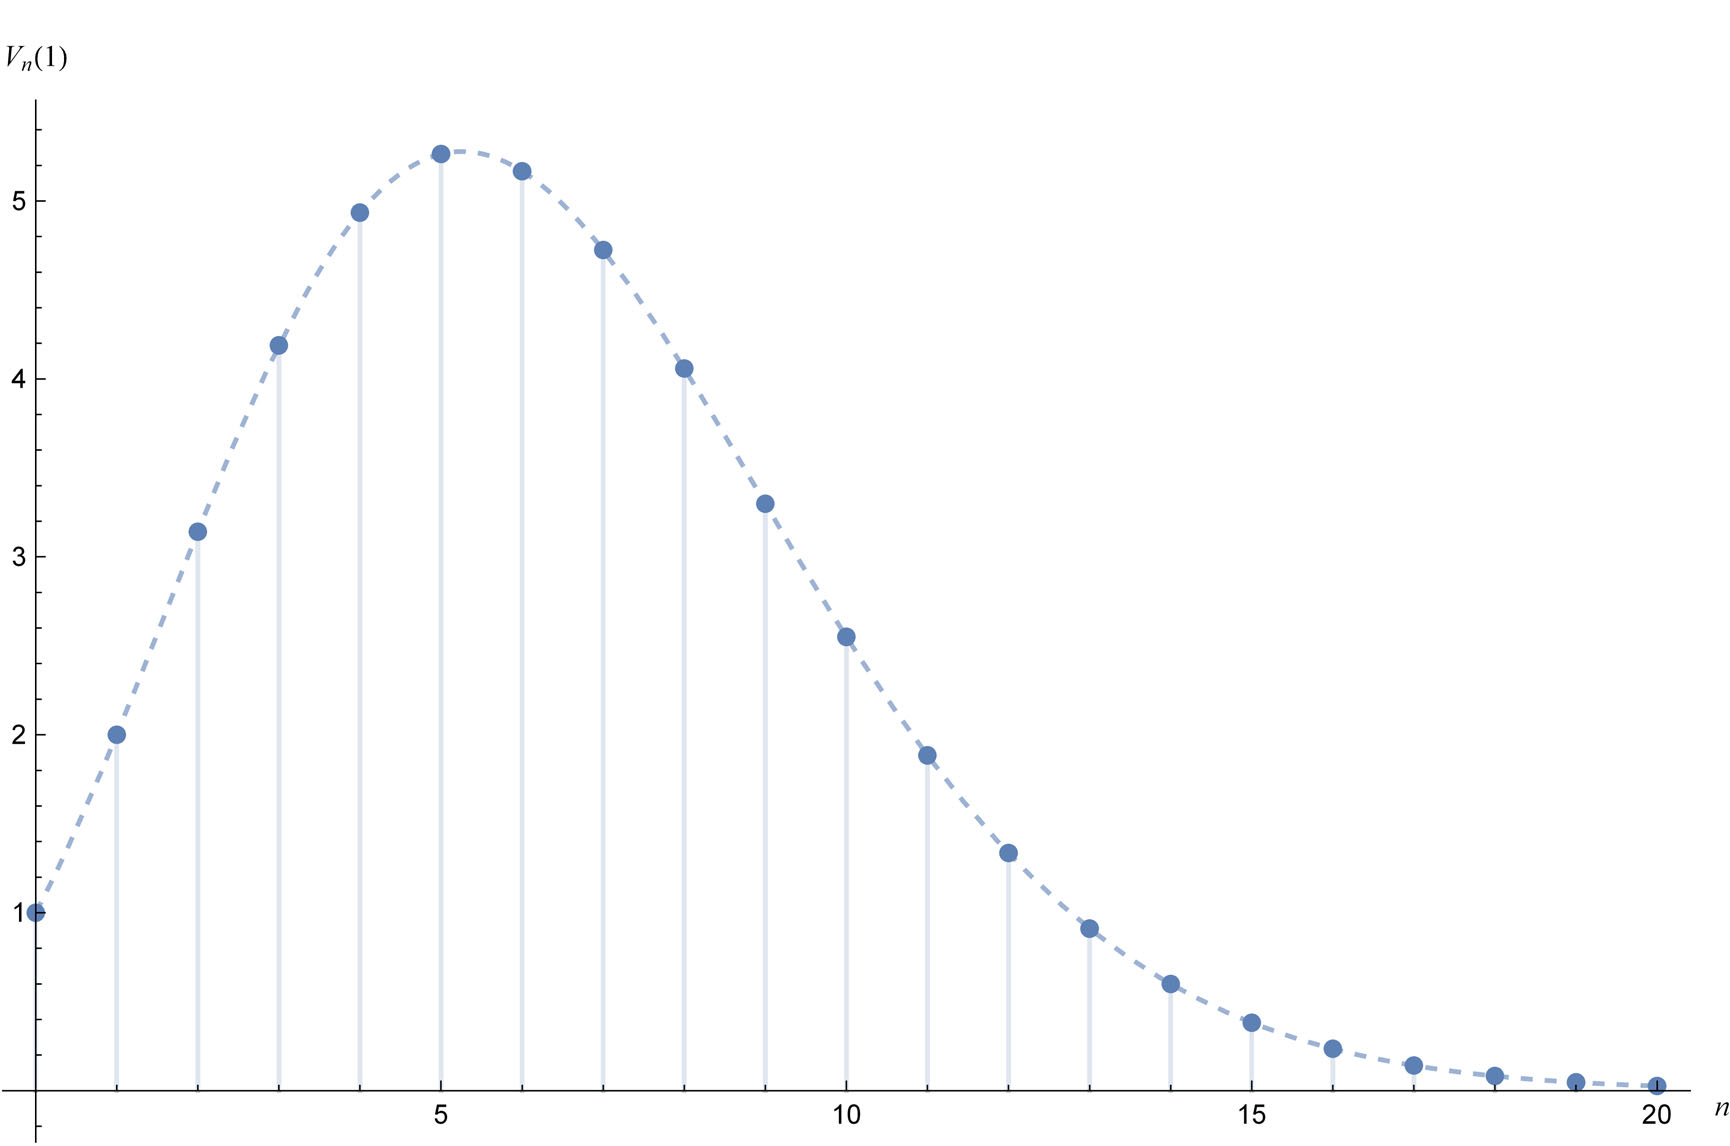
\includegraphics[width=0.75\textwidth]{figures/V_n(1).jpg}
		\caption{$V_n(1)$随$n$的变化关系}\label{fig:V_n(1)}
	\end{figure}

	\begin{figure}[h]
		\centering
		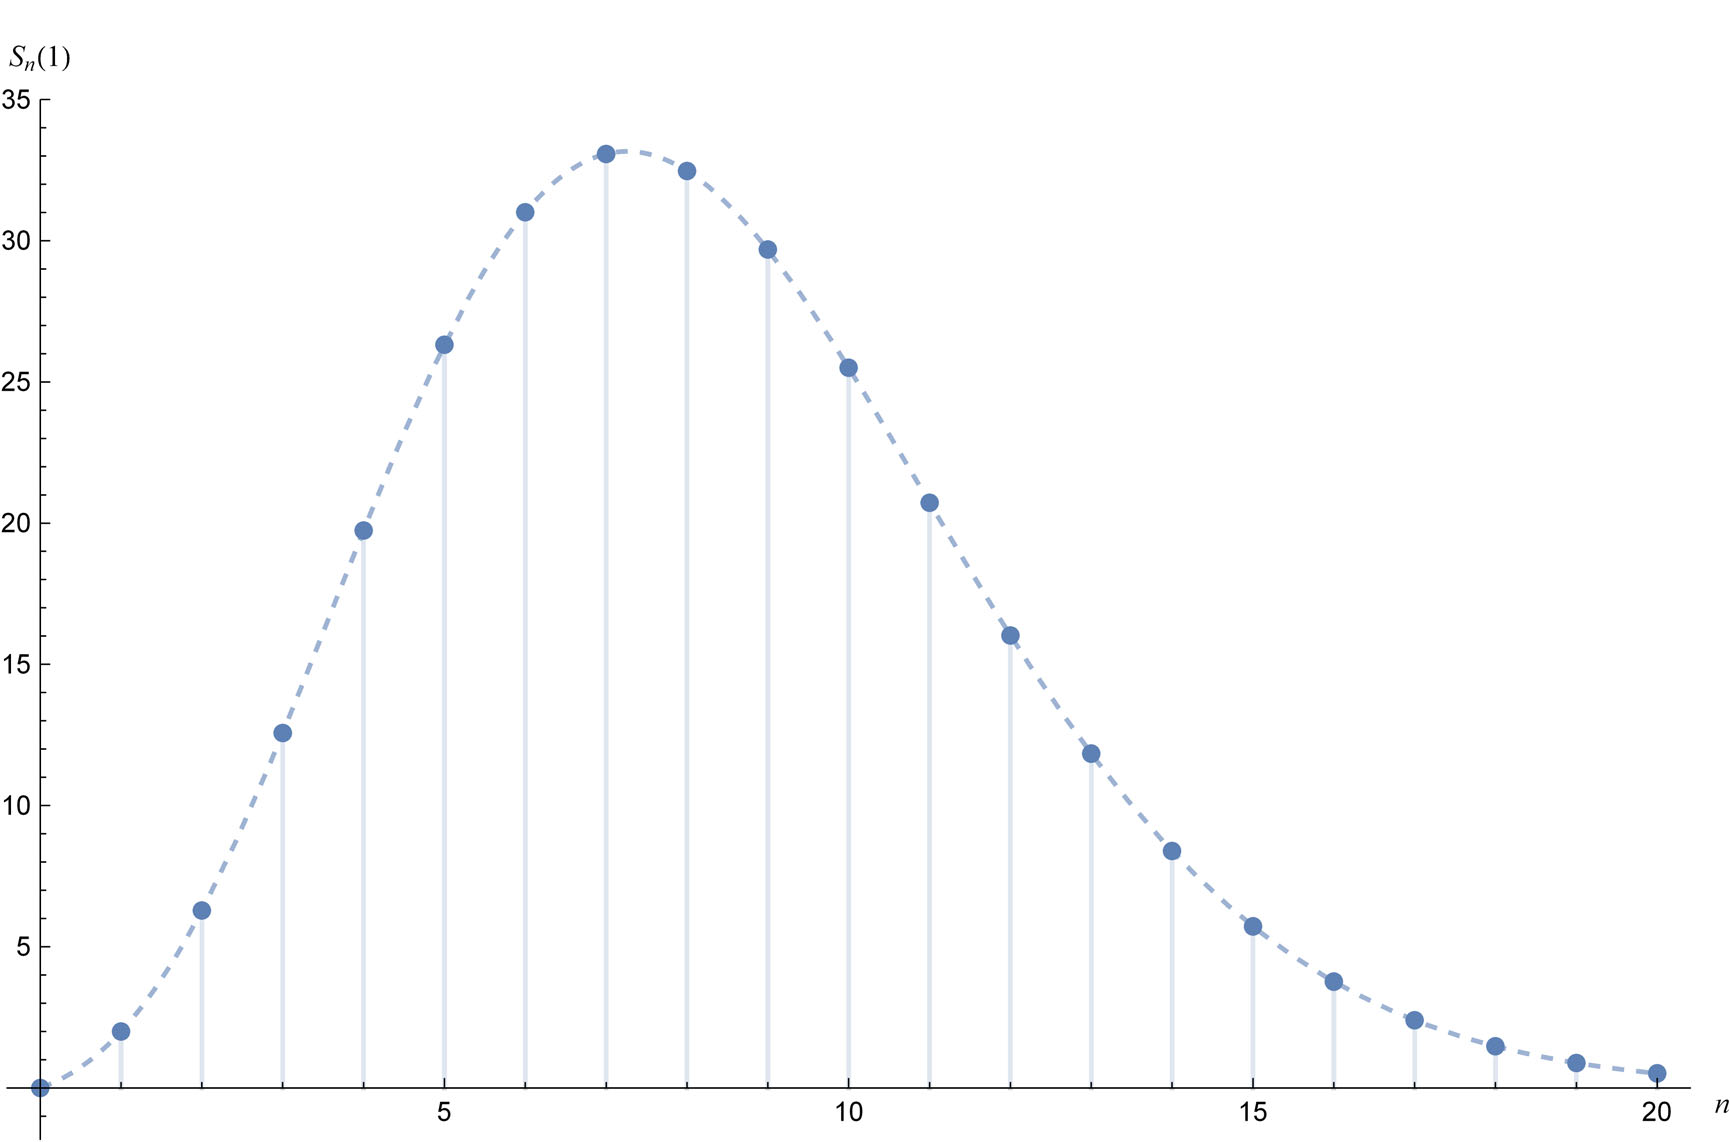
\includegraphics[width=0.75\textwidth]{figures/S_n(1).jpg}
		\caption{$S_n(1)$随$n$的变化关系}\label{fig:S_n(1)}
	\end{figure}
	可以看到,当$n=5$时,单位球的体积最大;当$n=7$时,单位球的表面积最大.而随着维数$n$不断增大,单位球的体积、表面积却在趋于零,这种现象源于Gamma函数的增长速度远大于指数函数.

	高维球还产生了一些有趣的问题,例如高维空间的最密堆积问题.目前这一问题还没有通解.另外,我们还可以引入Hausdorff维数,使得$n$的取值范围从正整数集扩大到实数集,此时又会产生怎样的新问题?
	
	\newpage
		\newpage
	
\end{document}


%\begin{equation}  公式居中编号
%	\begin{split}
		
%	\end{split}
%\end{equation}

%\notag  某行公式不编号